\documentclass[11pt,a4paper,oneside]{report}
\usepackage{pslatex,palatino,avant,graphicx,color,hyperref}
\usepackage{amsmath}
\usepackage{amsfonts}
\usepackage{amssymb}
\usepackage{framed}
\usepackage{minted}
\usepackage[margin=2cm]{geometry}
\usepackage{simpsons}

\hypersetup{
colorlinks=true,
linkcolor=blue,
linktoc=section,
urlcolor=blue
}

\begin{document}
\title{\it\huge Elements of Scientific Computing in Julia}
\maketitle

\tableofcontents
\newpage

\section*{Lecture 1}
\addcontentsline{toc}{section}{Lecture 1}

{\center\color{magenta}
\subsection*{{\it\huge What is Scientific Computing?}}}
\addcontentsline{toc}{subsection}{What is Scientific Computing?}

{\it\huge S}cientific computing is the process of coming up with algorithms and computer programs to solve quantitative and qualitative problems arising in areas such as the engineering and behavioral sciences, as well as biology and finance.\\

As a scientist of a specific area, one might develop a formula for making predictions. In general, these formulas will have several variables, so that an analytic solution might be difficult or even impossible to find. Scientists must then rely on computers to find a combination of variables that will produce a good approximation to the solution of a given problem. Scientific computing will draw heavily from two subjects: mathematics and computer science. We need the mathematics to come up with a well defined mathematical model to solve a particular science problem, but we will also need computer science to design robust, precise and well performing algorithms as well as recognize the correct tools to use, since the concern for optimal approximate solutions rely heavily on precision and performance.\\

Usually, scientific  problems are concerned with approximate and quantitative results to continuous (or numerical) problems. This course will take a broader view of what is usually covered in most scientific computing courses. It also includes topics from statistical learning and data analysis, therefore at times we will also be concerned with qualitative solutions and discretely modeled problems. Some examples of scientific computing tools and problems we will be studying are: \\

\begin{enumerate}
\item Numerical Integration: algorithms for computing the numerical value of definite integrals, such as the trapezoidal and Simpson's rule. As you know the definite integral of a given function can be interpreted as the area under the curve. There is several reasons a scientist may need to take an integral: calculating force, calculating errors, sampling, etc. Not all functions are easy to integrate analytically, thus numerical integration can be used to find approximate results. We will explore simple numerical integration problems as an introduction to Julia.

\item Stencil Computation: algorithms for computing the numerical solution to partial differential equations. As an example we will learn about the heat equation, its discretization, and ways to solve it numerically. The heat equation is a partial differential equation describing the distribution of heat in a given region over time.

\item Numerical Linear Algebra: algorithms for matrix factorization and for solving systems of linear equations. We will focus on solving the linear least squares problem for linear regression analysis of data sets.

\item Numerical Optimization: gradient decent algorithm for finding local minimum of a function. We will go back to the problem of solving systems of linear equations via linear least squares and reformulate it as a quadratic minimization problem.

\item Logistic Regression: a qualitative form of regression analysis aiming to separate or classify a data set into qualitative (discrete) categories. We will focus on the binary case and work on classification algorithms for separating spam from ham.

\item And Many More..: other topics and examples that are relevant to scientific computing are recommender systems, sentiment analysis, solving non-linear systems of equations, parallel computing and high performance computing. As an overview course, we will have a chance to discuss many topics of these topics at a high level.\\
\end{enumerate}

\newpage
A computational scientist must be well versed with an efficient and easy to use programming language, so that he may constantly change his program in search of better results. In this course we will use Julia, a high performing and dynamic programming language. It's syntax is friendly and flexible for programming scientific computing algorithms. Julia's compiler is based on the LLVM (Low Level Virtual Machine) compiler infrastructure, so performance is not an issue. Here are some benchmarks for comparison:\\

\begin{center}
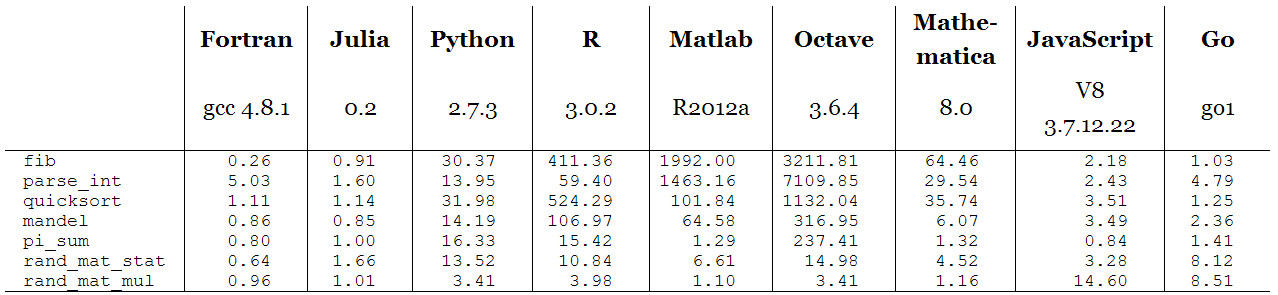
\includegraphics[width=6in]{benchmarksJulia.png}
\end{center}

More information on Julia can be found at \href{http://julialang.org/}{julialang.org}\\

Finally, two other important aspects of scientific computing are presentation and collaboration. It is not enough for scientists to come up with formulas and long tables of coefficients obtained computationally. Scientists must make sense of it all and present their results in a clean, standard and modular format via the use of tools such as \LaTeX $\;$ (for typesetting documents) and Git (for revision control). Many other presentation and collaboration tools exist, but in this course we will cover the the aforementioned ones.\\

{\center\color{magenta}
\subsection*{{\it\huge Installation and Tools Set-up}}}
\addcontentsline{toc}{subsection}{Installation and Tools Set-up}

{\it\huge O}ur computational scientist's tool box will consist of the following: \\
\begin{enumerate}
\item {\it\large Mathematical tools}: through out the course I will be assigning required reading of freely available documents as well as optional non-free resources on the mathematical tools necessary for arriving at the solutions of many interesting scientific problems. There is no required textbook for this class, however I would like to recommend Michael Heath's {\it Scientific Computing: An Introductory Survey} as an appropriate textbook for this course if you wish to acquire one. These lecture notes, as well as the homework assignments found herein, are significantly inspired by Heath's textbook.

\item {\it\large Julia}: this is the programming language we will use in the classroom and for the homework assignments. You will need to install Julia on your machine. Please follow the instructions below.

\item {\it\large Git}: this is a revision (or version) control and source code management system focused on speed, originally created in 2005 by Linus Torvalds for Linux kernel development, now widely used for sharing source code and keeping track of different versions of computer programming projects.  You will need to install Git on your machine. Please follow the instructions below.

\item {\it\large GitHub}: this is a web-based hosting service for computer programming projects using the Git RCS. We will be using GitHub as our class website, that is, there you will find our syllabus and homework descriptions. You will also submit your homework via Git on GitHub. First sign-up for a free public GitHub account at \href{https://github.com/}{github.com} with your \emph{.edu} address, then send me an email with your user name so that I may provide you with a free private repository for use in this class. 

\item \LaTeX $\;$(pronounced lay-tech): this is a document markup language that uses the \TeX $\;$ typesetting program for formatting text output, it is widely used in academia and for presenting mathematical formulas on various websites. Its philosophy is that authors should focus on the contents of their writing rather than getting distracted on the organization and structure of their document (\LaTeX $\;$ does it all for you, although getting distracted is possible). Installation instructions can be found below.\\
\end{enumerate}

{\it\large\color{red} Installing Julia:}
\begin{enumerate}
\item If you have a Mac or a Windows machine, download the \href{http://continuum.io/downloads}{Anaconda package} and run its installer. If you have a Linux machine, then install \href{http://ipython.org/install.html}{IPython} and related scientific-Python packages (SciPy and Matplotlib).

{\bf Important}! on Windows, the Anaconda installer will give you the following options: "Add Anaconda to the System Path" and also "Register Anaconda" as default Python version of the system. Make sure those boxes are selected.

\item Download Julia version 0.2 and run the installer. Do not download version 0.1. Then run the Julia application (double-click on it); a window with a \verb+julia>+ prompt will appear. At the prompt, type:

\begin{verbatim}
Pkg.add("IJulia")
Pkg.add("PyPlot")
\end{verbatim}

\item We will get started with IJulia in the section below.\\
\end{enumerate}

{\it\large\color{red} Installing Git:} 
\begin{itemize}
\item[] Please follow the instructions found at the  \href{https://help.github.com/articles/set-up-git}{Set Up Git} page of GitHub, for installing and setting up Git on your operating system. To get started using Git, you may want to either install the easy-to-use GUI provided by GitHub or go through this short and simple \href{http://rogerdudler.github.io/git-guide/}{tutorial}.\\
\end{itemize}

{\it\large\color{red} Installing \TeX :}
\begin{enumerate}
\item If you have a Mac, you will need to install \href{https://www.tug.org/mactex/}{MacTeX}. If you have Windows, you will have to install \href{http://www.miktex.org/download}{MikTeX}. If you have Linux, simply \verb+sudo apt-get install texlive+

\item You will also need a suitable editor for typesetting your documents. You are welcome to use your preferred editor, however I would like to recommend \href{http://www.xm1math.net/texmaker/download.html}{Texmaker} as a fairly easy editor to get started with \LaTeX.

\item You may want to go through this \href{http://www.maths.tcd.ie/~dwilkins/LaTeXPrimer/}{Getting Started with \LaTeX} guide, before starting to work on your first homework. Or you can always consult a \href{http://en.wikibooks.org/wiki/LaTeX/}{wiki} to find the command that does what you need, when you need it.\\
\end{enumerate}
\newpage

{\center\color{magenta}
\subsection*{{\it\huge Approximations, Errors and Getting Started with IJulia}}}
\addcontentsline{toc}{subsection}{Approximations, Errors and Getting Started with IJulia}

{\it\huge S}cientific computing is all about approximations, and approximations produce errors! The source of inexactness can come from any stage in the process of formulating and solving a scientific computing problem. We may be using a simplified model (since there are many complexities in real world problems that are difficult to account for); our measurement equipment have finite precision or we were not able to gather that much data anyway; we may have to discretize a continuous problem in order to solve it; truncation and rounding will happen due to computer precision. Therefore the accuracy of our final result will depend on a combination of all of these errors and approximations. We must study their effect on our results in order to better understand our results. Such study is called \emph{error analysis}.\\

{\bf Example 1 } Consider computing the surface area of the Earth by using the formula: $A = 4\pi r^2$.\\
\begin{itemize}
\item This formula gives the surface area of a perfect sphere, which is not necessarily the true shape of the Earth;
\item The radius of the Earth is based on a combination of measurements taken by equipment of finite precision;
\item $\pi$ is a transcendental infinite quantity, but it will have to be truncated at some point;
\item The final result will be rounded by our computers depending on their precision.\\
\end{itemize}

The stereotypical scientific computing problem can be view as computing the value of a function $f: \mathbf{R} \rightarrow \mathbf{R}$ (actually most scientific computing problems will be multidimensional, but let us consider one dimension for now). If we denote the true value of the input data by $x$, the true result by $f(x)$, the inexact input by $\hat{x}$ and the approximated function by $\hat{f}$, then:\\

Total Error = $\hat{f}(\hat{x}) - f(x) = (\hat{f}(\hat{x}) - f(\hat{x})) + (f(\hat{x}) - f(x))$  = computational error + propagated data error.\\

That is, the difference between using the approximate function and the exact function on the same input is a \emph{computational error}. While the difference between using the exact function on inexact input versus exact input is called a pure \emph{data error}.\\

Computational errors will be either truncation or rounding errors. Data errors may have more to do with other biases or limitations in collecting the data. \emph{Truncation error} is the difference between the result we get after truncating an infinite series (or other infinite quantities) and the result that would be produced if we were to use exact arithmetic. \emph{Rounding error} is the difference between the result we get due to using finite precision computers and the result that would be produced if we were to use exact arithmetic. Thus, \emph{computational error} is the sum of these two errors.\\

We can represent errors from numerical computations in either \emph{absolute} or \emph{relative} form:
\begin{center}
\emph{Absolute error} = approximate value - true value\\
\emph{Relative error} = (approximate value - true value)/true value
\end{center}

Note that the relative error can be seen as a percentage of the true value, if we multiply it by 100.\\

Besides analyzing the error of a approximate solution, it is also wise to understand the conditioning of our model. A problem is \emph{well-conditioned} if a relative change in the input date causes a similar relative change in the solution. While an \emph{ill-conditioned} problem is one where a relative change in the input data causes a much larger relative change in the solution. Given these definitions, we can calculate the condition number of a problems as follows (we denote it by $\mathcal{K}$):
\[\mathcal{K} = \frac{|\textnormal{relative change in solution}|}{|\textnormal{relative change in input data}|} = \frac{|(f(\hat{x})-f(x))/f(x)|}{|(\hat{x}-x)/x|}\]

{\bf Example 2 } Consider the problem of computing the values of $y = \cos(x)$ near $\pi/2$. Let $x = \pi/2$ and let $h$ be a small perturbation to $x$. Then we have:
\begin{center}
\emph{Absolute error} = $\cos(x+h) - \cos(x) \approx -h\sin(x) \approx -h$
\end{center}
This follows by the definition of the derivative: $\displaystyle f'(x) = \lim\limits_{h \rightarrow 0} \frac{f(x+h) - f(x)}{h}$. Recall that the derivative of $\cos(x)$ is $-\sin(x)$.
\begin{center}
\emph{Relative error} = $\displaystyle\frac{\cos(x+h) - \cos(x)}{\cos(x)} \approx -h\frac{\sin(x)}{\cos(x)} = -h\tan(x) \approx \infty$
\end{center}
Note that a small change in the input data for $\cos(x)$ near $\pi/2$, causes a large relative change in the output, regardless of how we computed it.

\begin{center}
\line(1,0){250}
\end{center}

Now let us explore errors and learn a bit of Julia using IJulia! Once you have followed the installation steps above, open up the command line and type:
\begin{verbatim}
ipython notebook --profile julia
\end{verbatim}

{\bf Important: }On Windows, you must run the above command from the \verb+bin+ subdirectory of the Julia directory that you downloaded/unpacked.\\

A dashboard window will open in your web browser. Click on the ``New Notebook'' button to start a new notebook. A notebook will combine code, computed results, formatted text, and images; for example, you might use one notebook for each problem set. You can click the ``Untitled0'' at the top to change the name, e.g. to ``Homework One''. You can enter Julia code at the \verb+In[ ]+ prompt, and hit {\bf shift-return} to execute it and see the results. If you hit {\bf return} without the {\bf shift} key, it will add additional lines to a single input cell. \\

{\bf Example 3 } On the next page, you can see what IJulia will look like in your browser. We can assign variables like \verb+r+ and \verb+A+ ({\bf note:} that no type is needed as Julia is dynamically typed). We can use the package \verb+PyPlot+ we installed earlier and plot some concentric circles.\\

Let us now work on a more relevant example...\\

\begin{center}
\includegraphics[width=7in]{IJuliaFirst.png}
\end{center}

\newpage
{\bf Example 4 } Let's write a Julia program to compute the mathematical constant e, the base of natural logarithms, from the definition:
\[ e = \lim\limits_{n \rightarrow \infty} (1+1/n)^n \]
We will compute $(1 + 1/n)^n$ for $n = 10^k$, $k = 1, 2, ..., 20$. Our goal will be to determine the error in the successive approximations we get by comparing them with the value of the built in constant $e$. A question for us to think about: do you think the error always decreases as n increases? \\

If we enter the following code into IJulia:\\
\definecolor{bg}{rgb}{0.95,0.95,0.95}
\begin{minted}[bgcolor=bg]{julia}
for k = 1:20
    a = (1+1/(10^k))^(10^k)
    err = a - e
    @printf("For k = %d, we get the approximation: %1.12f and the error %1.12f \n", 
    k, a, err)
end
\end{minted}

Then we will get the following result:
\begin{verbatim}
For k = 1,  we get the approximation: 2.593742460100 and the error -0.124539368359 
For k = 2,  we get the approximation: 2.704813829422 and the error -0.013467999038 
For k = 3,  we get the approximation: 2.716923932236 and the error -0.001357896223 
For k = 4,  we get the approximation: 2.718145926825 and the error -0.000135901634 
For k = 5,  we get the approximation: 2.718268237192 and the error -0.000013591267 
For k = 6,  we get the approximation: 2.718280469096 and the error -0.000001359363 
For k = 7,  we get the approximation: 2.718281694132 and the error -0.000000134327 
For k = 8,  we get the approximation: 2.718281798347 and the error -0.000000030112 
For k = 9,  we get the approximation: 2.718282052012 and the error  0.000000223553 
For k = 10, we get the approximation: 2.718282053235 and the error  0.000000224776 
For k = 11, we get the approximation: 2.718282053357 and the error  0.000000224898 
For k = 12, we get the approximation: 2.718523496037 and the error  0.000241667578 
For k = 13, we get the approximation: 2.716110034087 and the error -0.002171794372 
For k = 14, we get the approximation: 2.716110034087 and the error -0.002171794372 
For k = 15, we get the approximation: 3.035035206549 and the error  0.316753378090 
For k = 16, we get the approximation: 1.000000000000 and the error -1.718281828459 
For k = 17, we get the approximation: 1.000000000000 and the error -1.718281828459 
For k = 18, we get the approximation: 1.000000000000 and the error -1.718281828459 
For k = 19, we get the approximation: 1.000000000000 and the error -1.718281828459 
For k = 20, we get the approximation: 1.000000000000 and the error -1.718281828459 
\end{verbatim}

Note that we get the smallest error at $k = 8$, and then the error starts to increase again. When we reach $k=16$ the error is pretty large, and after that the approximation is \verb+1.000000000000+, which is quite wrong! A good discussion or personal research topic is to figure out why this is happening when it is happening.
\newpage
{\center\color{magenta}
\subsection*{{\it\huge Homework 1 (C)}}}
\addcontentsline{toc}{subsection}{Homework 1 (C)}

{\it\huge T}he purpose of homework 1 is for you to become better acquainted with the software tools you will be using this quarter as well as check your understanding of what is scientific computing and how do errors of various types arise in this field. \\

{\bf Exercises: }
\begin{enumerate}
\item (5 pts) Read the following \href{http://www.ee.columbia.edu/~dpwe/e6891/resources/1210.0530v3.pdf}{paper} and write a 1-2 pages summary using \LaTeX $\;$ formatting. Include at least one (numbered or bullet) list, a boldfaced/italicized/underlined sentence, a mathematical formula and a snippet of source code.

\item (5 pts) Solve the following problem using IJulia: If an amount $a$ is invested at interest rate $r$ compounded $n$ times per year, the the final value $f$ at the end of one year is given by $f = a(1 + r/n)^n$. This is the familiar formula for compound interest (so if we compound annually, then $n=1$). Typically, compounding is done quarterly ($n=4$) or daily ($n=365$). Note that the more we compound the greater the final amount at the end of the year, since more interest is paid on top of previous interest. But how much difference does this frequency actually make? \\

Write a program that implements the compound interest formula. Test your program using an initial investment of $a=100$, and interest rate of 5 percent (i.e. $r=0.05$), and the following values for $n$: 1, 4, 365, 10,000, and 20,000. Implement the compound interest formula in two different ways:
\begin{enumerate}
\item[a) ] using a loop that repeatedly multiplies $a$ by $(1+r/n)$ for a total of $n$ times; and
\item[b) ] using built-in exponentiation and logarithms (note that in this case the compound interest formula can be re-written as such: $f = ae^{n\ln(1+r/n)}$).
\end{enumerate}
Compare your results from both parts a and b and write a few comments about the comparison in a comment block within your source code.

\item (5 pts) Solve the following exercises and submit your answers in a pdf file using any formatting (+2 points for using \LaTeX $\;$ formatting):
\begin{enumerate}
\item[a) ]What are the approximate absolute and relative errors in approximating $\pi$ by each of the following quantities? 
\begin{enumerate}
\item[i) ]3
\item[ii) ]3.14
\item[iii) ]22/7
\end{enumerate}
\item[b) ]Consider the problem of evaluating the function $\sin(x)$, in particular, the propagated data error, i.e., the error in the function value due to a perturbation $h$ in the argument $x$.
\begin{enumerate}
\item[i) ]Estimate the absolute error in evaluating $\sin(x)$.
\item[ii) ]Estimate the relative error in evaluating $\sin(x)$.
\item[iii) ]Estimate the condition number for this problem.
\item[iv) ]For what values of the argument $x$ is this problem highly sensitive?\\
\end{enumerate}
\end{enumerate}
\end{enumerate}

{\bf Note: }This homework is due one week after it has been assigned and it should be turned in via your private GitHub repository for this class.
\newpage


\section*{Lecture 2}
\addcontentsline{toc}{section}{Lecture 2}

{\center\color{magenta}
\subsection*{{\it\huge Programming with Julia}}}
\addcontentsline{toc}{subsection}{Programming with Julia}

{\it\huge T}his lecture is meant as a crash course in Julia, a scientific computing language developed at MIT. Julia is a high-level, high-performance, dynamic programming language. This means that you can spend more time worrying about your scientific computing problems and models, rather than providing detailed computer instructions in your code. Some of the benefits of using Julia are:\\
\begin{itemize}
\item Julia is free and open source;
\item Unlike MATLAB, de-vectorized code is fast;
\item Julia is well equipped for parallel computing;
\item We can call C functions directly;
\item Power type system - support for arbitrary precision.\\
\end{itemize}

If you want to learn more details about Julia's history and features, I highly recommend reading this paper: \href{http://julialang.org/images/julia-dynamic-2012-tr.pdf}{Julia: A Fast Dynamic Language for Technical Computing}.\\

Now on to the crash-course! ({\bf Note:} This is a summary/selective copy-paste of the \href{http://learnxinyminutes.com/docs/julia/}{Learn X=Julia in Y Minutes} page. For a more detail tutorial, you may find \href{http://docs.julialang.org/en/release-0.2/manual/}{The Julia Manual} useful).
\begin{verbatim}
# Single line comments start with a hash.

####################################################
## 1. Primitive Datatypes and Operators
####################################################

# Everything in Julia is an expression.

# There are several basic types of numbers.
3 #=> 3 (Int64)
3.2 #=> 3.2 (Float64)
2 + 1im #=> 2 + 1im (Complex{Int64})
2//3 #=> 2//3 (Rational{Int64})

# All of the normal infix operators are available.
1 + 1 #=> 2
8 - 1 #=> 7
10 * 2 #=> 20
35 / 5 #=> 7.0
5 / 2 #=> 2.5 # dividing an Int by an Int always results in a Float
div(5, 2) #=> 2 # for a truncated result, use div
5 \ 35 #=> 7.0
2 ^ 2 #=> 4 # power, not bitwise xor
12 % 10 #=> 2

# Enforce precedence with parentheses
(1 + 3) * 2 #=> 8



# Boolean values are primitives
true
false

# Boolean operators
!true #=> false
!false #=> true
1 == 1 #=> true
2 == 1 #=> false
1 != 1 #=> false
2 != 1 #=> true
1 < 10 #=> true
1 > 10 #=> false
2 <= 2 #=> true
2 >= 2 #=> true
# Comparisons can be chained
1 < 2 < 3 #=> true
2 < 3 < 2 #=> false

# Strings are created with "
"This is a string."

# Character literals are written with '
'a'

# A string can be indexed like an array of characters
"This is a string"[1] #=> 'T' # Julia indexes from 1
# However, this is will not work well for UTF8 strings,
# so iterating over strings is recommended (map, for loops, etc).

# $ can be used for string interpolation:
"2 + 2 = $(2 + 2)" #=> "2 + 2 = 4"
# You can put any Julia expression inside the parenthesis.

# Another way to format strings is the printf macro.
@printf "%d is less than %f" 4.5 5.3 # 5 is less than 5.300000

# Printing is easy
println("I'm Julia. Nice to meet you!")


####################################################
## 2. Variables and Collections
####################################################

# Variable names start with a letter.
# After that, you can use letters, digits, underscores, and exclamation points.
SomeOtherVar123! = 6 #=> 6

# You don't declare variables before assigning to them.
some_var = 5 #=> 5
some_var #=> 5

# Accessing a previously unassigned variable is an error
try
    some_other_var #=> ERROR: some_other_var not defined
catch e
    println(e)
end

# Arrays store a sequence of values indexed by integers 1 through n:
a = Int64[] #=> 0-element Int64 Array

# Note that arrays must be given a type, and all elements in the array
must be of that type.

# 1-dimensional array literals can be written with comma-separated values.
b = [4, 5, 6] #=> 3-element Int64 Array: [4, 5, 6]
b[1] #=> 4
b[end] #=> 6

# 2-dimentional arrays use space-separated values and semicolon-separated rows.
matrix = [1 2; 3 4] #=> 2x2 Int64 Array: [1 2; 3 4]

# Add stuff to the end of an array with push! and append!
push!(a,1)     #=> [1]
push!(a,2)     #=> [1,2]
push!(a,4)     #=> [1,2,4]
push!(a,3)     #=> [1,2,4,3]
append!(a,b) #=> [1,2,4,3,4,5,6]

# Remove from the end with pop
pop!(b)        #=> 6 and b is now [4,5]

# Let's put it back
push!(b,6)   # b is now [4,5,6] again.

a[1] #=> 1 # remember that Julia indexes from 1, not 0!

# end is a shorthand for the last index. It can be used in any
# indexing expression
a[end] #=> 6

# we also have shift and unshift
shift!(a) #=> 1 and a is now [2,4,3,4,5,6]
unshift!(a,7) #=> [7,2,4,3,4,5,6]

# Function names that end in exclamations points indicate that they modify
# their argument.
arr = [5,4,6] #=> 3-element Int64 Array: [5,4,6]
sort(arr) #=> [4,5,6]; arr is still [5,4,6]
sort!(arr) #=> [4,5,6]; arr is now [4,5,6]

# You can initialize arrays from ranges
a = [1:5] #=> 5-element Int64 Array: [1,2,3,4,5]

# You can look at ranges with slice syntax.
a[1:3] #=> [1, 2, 3]
a[2:] #=> [2, 3, 4, 5]
a[2:end] #=> [2, 3, 4, 5]

# Remove elements from an array by index with splice!
arr = [3,4,5]
splice!(arr,2) #=> 4 ; arr is now [3,5]

# Check for existence in an array with in
in(1, a) #=> true

# Examine the length with length
length(a) #=> 8

# Tuples are immutable.
tup = (1, 2, 3) #=> (1,2,3) # an (Int64,Int64,Int64) tuple.
tup[1] #=> 1
try:
    tup[1] = 3 #=> ERROR: no method setindex!((Int64,Int64,Int64),Int64,Int64)
catch e
    println(e)
end

# Many array functions also work on tuples
length(tup) #=> 3
tup[1:2] #=> (1,2)
in(2, tup) #=> true

# You can unpack tuples into variables
a, b, c = (1, 2, 3) #=> (1,2,3)  # a is now 1, b is now 2 and c is now 3

# Tuples are created even if you leave out the parentheses
d, e, f = 4, 5, 6 #=> (4,5,6)

# Look how easy it is to swap two values
e, d = d, e  #=> (5,4) # d is now 5 and e is now 4

# Dictionaries store mappings
empty_dict = Dict() #=> Dict{Any,Any}()

# You can create a dictionary using a literal
filled_dict = ["one"=> 1, "two"=> 2, "three"=> 3]
# => Dict{ASCIIString,Int64}

# Look up values with []
filled_dict["one"] #=> 1

# Get all keys
keys(filled_dict)
#=> KeyIterator{Dict{ASCIIString,Int64}}(["three"=>3,"one"=>1,"two"=>2])
# Note - dictionary keys are not sorted or in the order you inserted them.

# Get all values
values(filled_dict)
#=> ValueIterator{Dict{ASCIIString,Int64}}(["three"=>3,"one"=>1,"two"=>2])
# Note - Same as above regarding key ordering.

# Check for existence of keys in a dictionary with in, haskey
in(("one", 1), filled_dict) #=> true
in(("two", 3), filled_dict) #=> false
haskey(filled_dict, "one") #=> true
haskey(filled_dict, 1) #=> false

# Trying to look up a non-existant key will raise an error
try
    filled_dict["four"] #=> ERROR: key not found: four in getindex at dict.jl:489
catch e
    println(e)
end

# Use the get method to avoid that error by providing a default value
# get(dictionary,key,default_value)
get(filled_dict,"one",4) #=> 1
get(filled_dict,"four",4) #=> 4

####################################################
## 3. Control Flow
####################################################

# Let's make a variable
some_var = 5

# Here is an if statement. Indentation is not meaningful in Julia, but
it is good for readability.

if some_var > 10
    println("some_var is totally bigger than 10.")
elseif some_var < 10    # This elseif clause is optional.
    println("some_var is smaller than 10.")
else                    # The else clause is optional too.
    println("some_var is indeed 10.")
end
#=> prints "some var is smaller than 10"


# For loops iterate over iterables.
# Iterable types include Range, Array, Set, Dict, and String.
for animal=["dog", "cat", "mouse"]
    println("$animal is a mammal")
    # You can use $ to interpolate variables or expression into strings
end
# prints:
#    dog is a mammal
#    cat is a mammal
#    mouse is a mammal

# You can use 'in' instead of '='.
for animal in ["dog", "cat", "mouse"]
    println("$animal is a mammal")
end
# prints:
#    dog is a mammal
#    cat is a mammal
#    mouse is a mammal

for a in ["dog"=>"mammal","cat"=>"mammal","mouse"=>"mammal"]
    println("$(a[1]) is a $(a[2])")
end
# prints:
#    dog is a mammal
#    cat is a mammal
#    mouse is a mammal

for (k,v) in ["dog"=>"mammal","cat"=>"mammal","mouse"=>"mammal"]
    println("$k is a $v")
end
# prints:
#    dog is a mammal
#    cat is a mammal
#    mouse is a mammal

# While loops loop while a condition is true
x = 0
while x < 4
    println(x)
    x += 1  # Shorthand for x = x + 1
end
# prints:
#   0
#   1
#   2
#   3

# Handle exceptions with a try/catch block
try
   error("help")
catch e
   println("caught it $e")
end
#=> caught it ErrorException("help")


####################################################
## 4. Functions
####################################################

# The keyword 'function' creates new functions
#function name(arglist)
#  body...
#end
function add(x, y)
    println("x is $x and y is $y")

    # Functions return the value of their last statement
    x + y
end

add(5, 6) #=> 11 after printing out "x is 5 and y is 6"

# You can define functions that take a variable number of
# positional arguments
function varargs(args...)
    return args
    # use the keyword return to return anywhere in the function
end
#=> varargs (generic function with 1 method)

varargs(1,2,3) #=> (1,2,3)

# The ... is called a splat.
# We just used it in a function definition.
# It can also be used in a fuction call,
# where it will splat an Array or Tuple's contents into the argument list.
Set([1,2,3])    #=> Set{Array{Int64,1}}([1,2,3]) # produces a Set of Arrays
Set([1,2,3]...) #=> Set{Int64}(1,2,3) # this is equivalent to Set(1,2,3)

x = (1,2,3)     #=> (1,2,3)
Set(x)          #=> Set{(Int64,Int64,Int64)}((1,2,3)) # a Set of Tuples
Set(x...)       #=> Set{Int64}(2,3,1)


# You can define functions with optional positional arguments
function defaults(a,b,x=5,y=6)
    return "$a $b and $x $y"
end

defaults('h','g') #=> "h g and 5 6"
defaults('h','g','j') #=> "h g and j 6"
defaults('h','g','j','k') #=> "h g and j k"
try
    defaults('h') #=> ERROR: no method defaults(Char,)
    defaults() #=> ERROR: no methods defaults()
catch e
    println(e)
end

# You can define functions that take keyword arguments
function keyword_args(;k1=4,name2="hello") # note the ;
    return ["k1"=>k1,"name2"=>name2]
end

keyword_args(name2="ness") #=> ["name2"=>"ness","k1"=>4]
keyword_args(k1="mine") #=> ["k1"=>"mine","name2"=>"hello"]
keyword_args() #=> ["name2"=>"hello","k1"=>4]

# You can combine all kinds of arguments in the same function
function all_the_args(normal_arg, optional_positional_arg=2; keyword_arg="foo")
    println("normal arg: $normal_arg")
    println("optional arg: $optional_positional_arg")
    println("keyword arg: $keyword_arg")
end

all_the_args(1, 3, keyword_arg=4)
# prints:
#   normal arg: 1
#   optional arg: 3
#   keyword arg: 4

# Julia has first class functions
function create_adder(x)
    adder = function (y)
        return x + y
    end
    return adder
end

# This is "stabby lambda syntax" for creating anonymous functions
(x -> x > 2)(3) #=> true

# This function is identical to create_adder implementation above.
function create_adder(x)
    y -> x + y
end

# You can also name the internal function, if you want
function create_adder(x)
    function adder(y)
        x + y
    end
    adder
end

add_10 = create_adder(10)
add_10(3) #=> 13


# There are built-in higher order functions
map(add_10, [1,2,3]) #=> [11, 12, 13]
filter(x -> x > 5, [3, 4, 5, 6, 7]) #=> [6, 7]

# We can use list comprehensions for nicer maps
[add_10(i) for i=[1, 2, 3]] #=> [11, 12, 13]
[add_10(i) for i in [1, 2, 3]] #=> [11, 12, 13]

\end{verbatim}

Hopefully, the brief tutorial above will give you most of the necessary Julia syntax knowledge for this quarter. One thing worth emphasizing is Julia's capabilities for arbitrary precision arithmetic. Recall the example we worked on in Lecture 1: \\

Write a Julia program to compute the mathematical constant e, the base of natural logarithms, from the definition:
\[ e = \lim\limits_{n \rightarrow \infty} (1+1/n)^n \]
Compute $(1 + 1/n)^n$ for $n = 10^k$, $k = 1, 2, ..., 20$ and determine the error in the successive approximations by comparing them with the value of the built in constant $e$.  \\

If we enter the following \emph{modified} code into IJulia:\\

\begin{minted}[bgcolor=bg]{julia}
for k = 1:2:20
    a = (1+BigFloat(1/10^k))^BigFloat(10^k)
    err = a - e
    @printf("For k = %d, we get the approximation: %1.12f and the error %1.12f \n", 
    k, a, err)
end
\end{minted}

We get the following output:
\begin{verbatim}
For k = 1,  we get the approximation: 2.593742460100 and the error -0.124539368359045110601357 
For k = 3,  we get the approximation: 2.716923932236 and the error -0.001357896223152721491140 
For k = 5,  we get the approximation: 2.718268237174 and the error -0.000013591284555344964105 
For k = 7,  we get the approximation: 2.718281692545 and the error -0.000000135914079087169091 
For k = 9,  we get the approximation: 2.718281827100 and the error -0.000000001359140743684725 
For k = 11, we get the approximation: 2.718281828445 and the error -0.000000000013591573606460 
For k = 13, we get the approximation: 2.718281828459 and the error -0.000000000000135831527022 
For k = 15, we get the approximation: 2.718281828459 and the error -0.000000000000001147915738 
For k = 17, we get the approximation: 2.718281828459 and the error  0.000000000000000180881062 
For k = 19, we get the approximation: 2.718281828459 and the error -0.000000000000000253747066
\end{verbatim}

Notice that I have chosen to loop from 1 to 20 with a step size of 2, this was just for the purpose of having a shorter output. You are welcome to inspect the output you get by using a step size of 1 as before. The main thing to notice in this modified version of our program is that we are using the \verb+BigFloat+ type. This means that we are now getting many more digits of accuracy than we were before and thus our results look pretty good and no longer seem to exhibit the imprecise behavior given larger values of $k$.

\begin{center}
\line(1,0){250}
\end{center}

Another great use for the Julia language is parallel computing. This is a big idea in scientific computing, which we may touch on this quarter, however a course that focuses primarily on high-performance and parallel computing is advised for those who wish more than just a honorable mention. 
\newpage

{\center\color{magenta}
\subsection*{\it\huge Numerical Integration: Concepts}}
\addcontentsline{toc}{subsection}{Numerical Integration: Concepts}

{\it\huge I}n your Integral Calculus class, you probably learned many different ways for analytically and algebraically solving for the definite integral of various different functions. That is, you were able to apply the Fundamental Theorem of Calculus to definite integrals and with some algebra you got an exact answer. However, you may have come across interesting integrable functions whose antiderivatives were difficult or even impossible to write, such as the famous probability density function for the normal distribution: $f(x)= \displaystyle \frac{1}{\sqrt{2 \pi}}e^{-x^2/2}$. In this lecture we will look at quadrature methods for solving one dimensional definite integrals numerically.\\

{\it\Large\color{red} Quadrature Methods}\\

Quadrature means to calculate the area, and as you may recall, the definite integral of a function can be interpreted as the area under the graph of the function within a particular interval. We can chop up the area of an unfamiliar shape into slices, and approximate the area of each slice with the area of a familiar shape (such as a rectangle or a trapezoid). If we add up the area of all these slices, we should get an approximation of the are under the given curve, and thus the approximate solution of the definite integral of the given function.\\

For all of the rules below consider the definite integral $\int\limits_a^b f(x) dx$, that is, the area under the curve $f$ in the closed interval $[a, b]$. We divide $[a, b]$ into $n$ subintervals of equal width $\Delta x = \frac{b - a}{n}$. \\
\begin{enumerate}
\item \emph{Midpoint Rule } - This rule obtains the area under the curve by subdividing the area into rectangles of equal width $\Delta x$ and height $f(x^*_i)$, where $x^*_i$ is the {\bf midpoint} of the subinterval $[x_{i-1}, x_i]$. \\ 

The area of each rectangle is then  $\displaystyle\Delta x f(x^*_i)$, and therefore, we get that: \\
\[ \int\limits_a^b f(x) dx \approx \Delta x f(x^*_1) + \Delta x f(x^*_2) + ... + \Delta x f(x^*_n)\]

\begin{center}
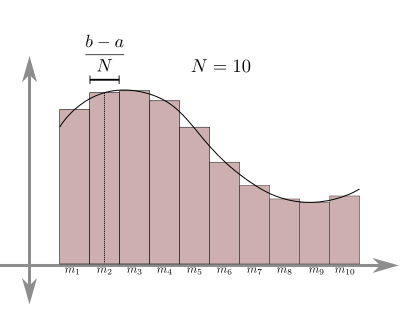
\includegraphics[width=2.5in]{MidpointRule.png}
\end{center}
\item \emph{Trapezoidal Rule } - This rule obtains the area under the curve by subdividing the area into trapezoids of equal trapezoidal height $\Delta x$, and base widths $f(x_{i-1})$ and $f(x_i)$ for each subinterval $[x_{i-1}, x_i]$. \\ 

The area of each trapezoid is then $\displaystyle\frac{\Delta x}{2}(f(x_{i-1}) + f(x_i))$, and therefore, we get that:\\
\[ \int\limits_a^b f(x) dx \approx \frac{\Delta x}{2}(f(x_0) + f(x_1)) + \frac{\Delta x}{2}(f(x_1) + f(x_2)) + ... + \frac{\Delta x}{2}(f(x_{n-1}) + f(x_n))\]
\begin{center}
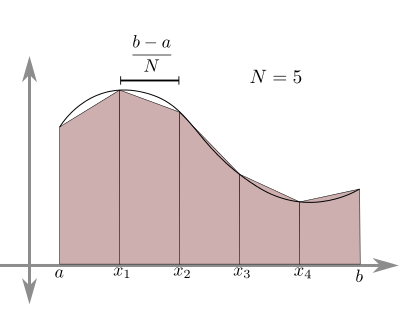
\includegraphics[width=2.5in]{TrapezoidRule.png}
\end{center}
\item \emph{Simpson's Rule} \Homer - This rule is an interpolative quadrature rule, since upon subdividing the curve into $n = 2k$ (that is, $n$ must be even) slices, we interpolate the best fit quadratic curve for each slice. Using Lagrange polynomial interpolation on the endpoints $a$, $b$ and the midpoint $m = (a+b)/2$, we find that the following quadratic function interpolates our curve on the interval $[a,b]$:
\[P(x) = f(a)\frac{(x-m)(x-b)}{(a-m)(a-b)} + f(m)\frac{(x-a)(x-b)}{(m-a)(m-b)} +f(b)\frac{(x-a)(x-m)}{(b-a)(b-m)} \]
With a bit of algebra and patience, it is easy to show that 
\[\int\limits_a^b P(x)dx = \frac{b-a}{6}\left[f(a) + 4f\left(\frac{a+b}{2}\right)+f(b)\right]\]
\begin{center}
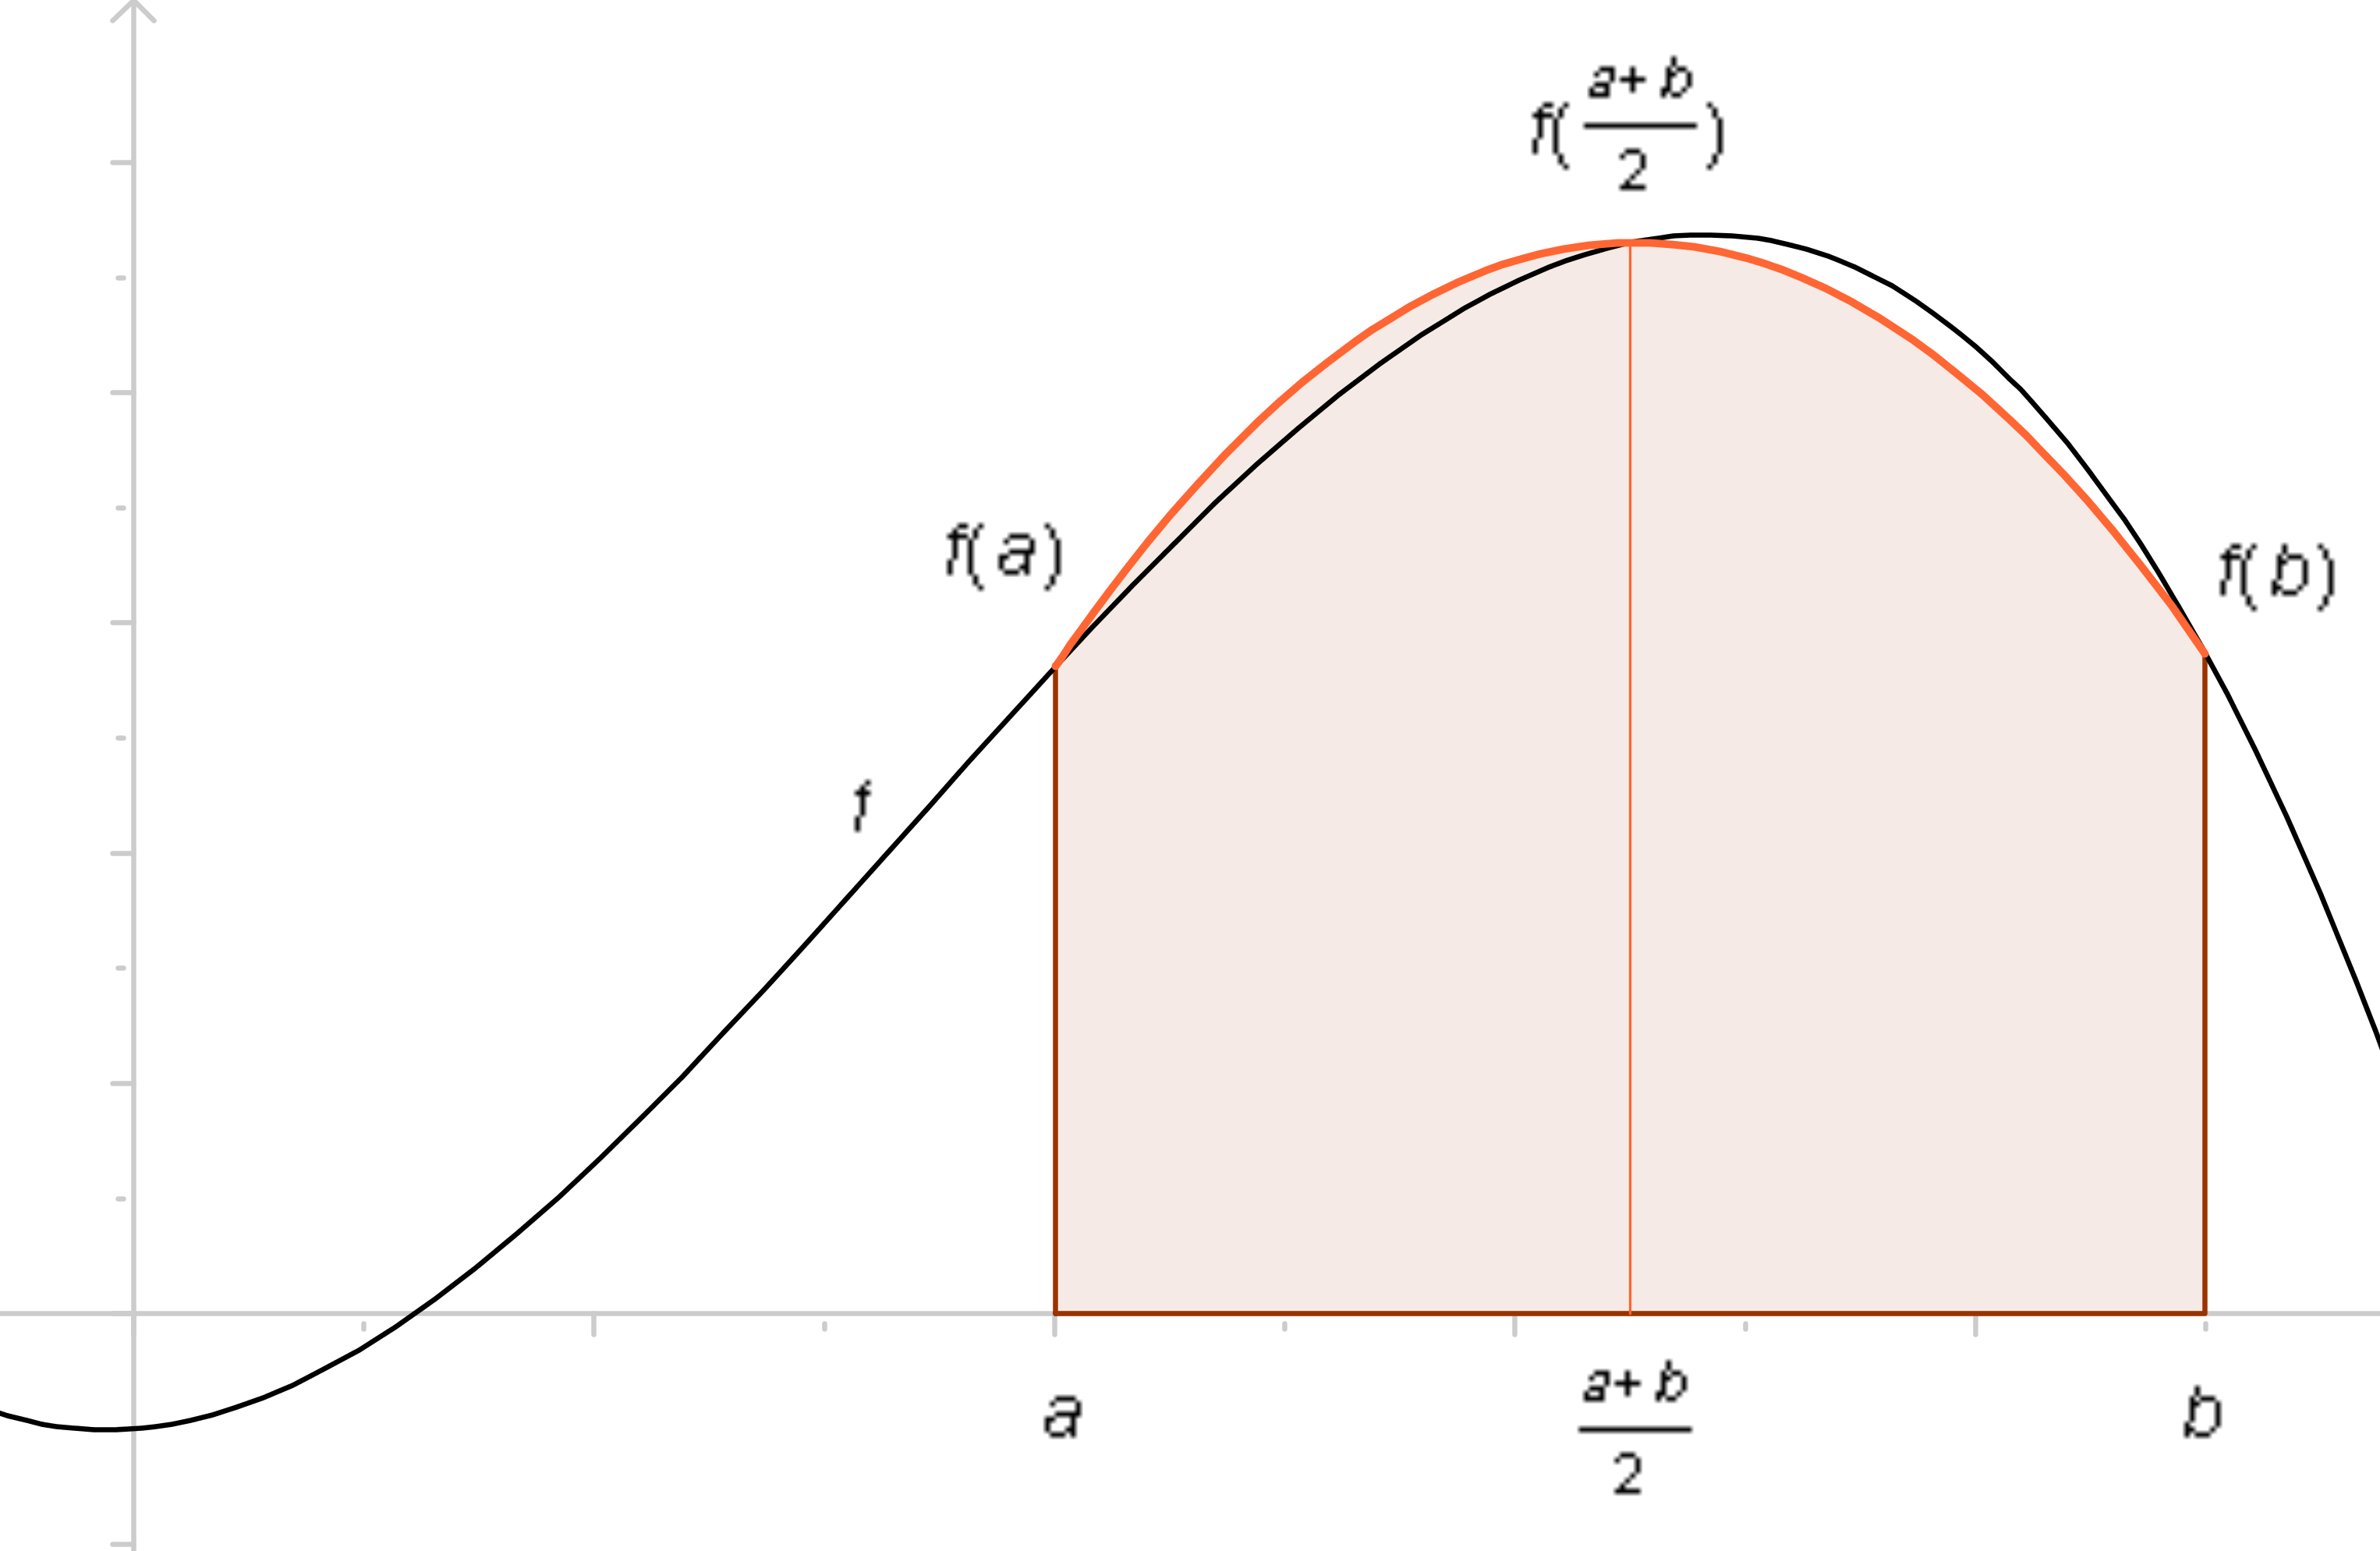
\includegraphics[width=2.5in]{SimpsonRule.png}
\end{center}
If subdivide the interval $[a,b]$ into $n = 2k$ sub-intervals, then the integral of $f(x)$ is approximately
\[\frac{\Delta x}{3}[f(x_0) + 4f(x_1) + 2f(x_2) + ... + 2f(x_{n-2}) + 4f(x_{n-1}) + f(x_n)] \]

\item \emph{Adaptive Quadrature} - this is a technique that can be used with any of the above rules and their respective error bounds (see next section). That is, we apply one of the above rules and if the error bound for a given interval is above a specified threshold, the algorithm then further subdivides the interval. Thus, the term $\Delta x$ is not fixed as before.\\
\end{enumerate}

Sources for the images: \url{http://calculus.seas.upenn.edu/?n=Main.DiscreteIntegration} and 
\url{https://en.wikipedia.org/wiki/Newton%E2%80%93Cotes_formulas}

\newpage
{\it\Large\color{red} Numerical Integration Error Bounds}\\

In the previous chapter we talked a great deal about errors and how important it is for computational scientists to understand the error caused by their mathematical models. We studied that error is equal to approximate value minus true value. Therefore, in other to determine the error of our numerical integration method, we can simply look at the difference between our result and the true result acquired via exact integration. That's easy! However, if we are able to get the true value, then why are we bothering with the approximation? \\

The cold truth is that for many problems we do not know the true value, but we can use mathematical theory to come up with upper bounds for our errors. \emph{Error bounds} are quantities we can easily compute (unfortunately, we will not discuss their derivation in this course - here is an \href{http://www.math.ucsd.edu/~ebender/20B/77_Trap.pdf}{optional reading} for the derivation of the trapezoidal rule error bound) and are set as ceilings for our errors, that is, the error obtained by a certain mathematical model is guaranteed to be less than its error bound. As you might have already guessed, an error bound depends on the mathematical model used (there is no universal error bound).\\

Below are the error bounds for the three methods of numerical integration we've discussed in this lecture. Let $f$ be the function we are numerically integrating. Suppose that $\max\limits_{a \leq x \leq b}|f''(x)| = K$ and $\max\limits_{a \leq x \leq b}|f^{(4)}(x)| = M$ for $a \leq x \leq b$, then:

\begin{enumerate}
\item \emph{The error bound for Midpoint Rule is}
\[\frac{K(b-a)^3}{24n^2}\]
\item \emph{The error bound for Trapezoidal Rule is}
\[\frac{K(b-a)^3}{12n^2}\]
\item \emph{The error bound for Simpson's Rule is}
\[\frac{M(b-a)^5}{180n^4}\]
\end{enumerate}

{\center\color{magenta}
\subsection*{\it\huge An Example: The Error Function}}
\addcontentsline{toc}{subsection}{An Example: The Error Function}

\[\textnormal{erf}(x) = \frac{2}{\sqrt{\pi}}\int\limits_0^xe^{-t^2}dt\]
The \href{http://en.wikipedia.org/wiki/Error_function}{error function} (occurring in statistics to measure the behavior of a sample with respect to the population mean) given above is an example of a non-elementary function - that is, we cannot express erf($x$) as a finite expression consisting of elementary operations (such as $+,-,\times,\div$) and components (such as logs, exponents, roots, and so on) . Thus it must be expressed as an integral, and if we desire to evaluate erf($x_0$), then we must evaluate the integral that defines erf in the interval $[0,x_0]$.\\

However, this is not a trivial task, as the above integral does not have an analytic solution. Therefore we must rely on numerical approximation techniques such as the numerical integration methods we've discussed in this lecture.\\

Let's use IJulia to implement the erf function using the midpoint rule. Our function will take two inputs: the upper bound $x$ of the interval of integration, and the number of sub-intervals $n$.\\
\newpage
\begin{minted}[bgcolor=bg]{julia}
# erf's integrand
function integrand(t)
    e^(-t^2)
end    

# erf function using the midpoint rule
# input: x - interval of integration upper bound, 
#        n - number of sub-intervals
# output: [erf(x), midpoint rule error bound]

function middle_erf(x, n)
    
    # calculate delta_x
    delta_x = x / n
   
    result = 0
    # summing up the are of rectangles
    for i = 1:n
        x_mid = ((i-1)*delta_x + i*delta_x)/2
        result += delta_x*integrand(x_mid)
    end
    result *= 2 / sqrt(pi)
    
    # since the SECOND derivative of e^(-t^2) is (4t^2 - 2)*(e^(-t^2)),
    # and since it obtains a maximum at t = sqrt(3/2) on the interval 
    # from 0 to x, when x greater than or equal to sqrt(3/2), OR just 
    # at t = x, when x < sqrt(3/2), then our K in the error bound
    # formula is:
    
    if x >= sqrt(3/2)
      error_bound = (4/e^(3/2))*(x^3)/(24*n^2)
    else 
      error_bound = abs((4*x^2 - 2)*(e^(-x^2)))*(x^3)/(24*n^2)
    end    
    
    return ["result" => result, "error bound" => error_bound]
end
\end{minted}
\newpage

{\center\color{magenta}
\subsection*{{\it\huge Homework 2 (P)}}}
\addcontentsline{toc}{subsection}{Homework 2 (P)}

{\it\huge T}he purpose of homework 2 is for you to continue becoming acquainted with the tools we will be using this quarter, as well as put into practice the integration techniques we have learned here. Also, I will be checking if you are using git as a revision system (as opposed to a homework submission system). Make sure you have finished homework 1 before embarking on a new homework adventure!\\

{\bf Exercises: }
\begin{enumerate}
\item (1 pt) In a \verb+.tex+ file (with appropriate mark-up) tell something about Julia I don't know. 
\item (8 pts) Implement a function in Julia called \verb+simp_erf+, which takes as input the {\bf upper bound of the integration interval} (that is, the ``$x$'' in the build-in erf($x$)) and an {\bf error bound} (that is, instead of giving the function the number of sub-intervals $n$ as in the lecture example, we should be able to give the error bound instead) in order to calculate the value given by the error function (erf) using the Simpson's Rule. Compare your results with those of \verb+middle_erf+ and write a few sentences about it using \LaTeX $\;$ (use the same \verb+.tex+ file as in exercise 1).

\item (2 pts each) Use numerical integration to verify or refute each of the following conjectures. Also, provide a plot of each integrand:
\begin{enumerate}
\item[a) ] $\displaystyle\int\limits_0^1 \sqrt{x^3} = 0.4$
\item[b) ] $\displaystyle\int\limits_0^{10} \frac{50}{\pi(2500x^2+1)}dx = 0.5$
\item[c) ] $\displaystyle\int\limits_{-9}^{100} \frac{1}{\sqrt{|x|}}dx = 26$
\end{enumerate}
\end{enumerate}
\begin{center}
\Lisa $>$ ``This homework is so much fun!''
\end{center} 
\newpage


\section*{Lecture 3}
\addcontentsline{toc}{section}{Lecture 3}

{\it \huge I}n this lecture we will talk about numerical differentiation. In particular, we will explore the discretization and numerical solutions of partial differential equations (or PDE's). Unlike integration (where we deal with multiplication and addition), differentiation (where we deal with differences and division) is a sensitive problem, as small perturbations in the data can cause large change in the results.\\

If we only know the values of a function we wish to differentiate at a discrete set of points, then we could try to fit a smooth curve through those points and differentiate this curve. However we must be careful, since interpolating the appropriate curve is often difficult, specially if our data set is very noisy. \\

There are several methods for numerically solving PDE's and there is no single best method to solve all PDE's. That is, which method you use to solve a particular problem will depend on the problem and the available data. In this lecture we will explore the finite difference method for solving PDE's. This is one of many other \href{https://en.wikipedia.org/wiki/Numerical_partial_differential_equations}{methods} I would encourage you to research on your own based on your interests.\\

{\center\color{magenta}
\subsection*{\it\huge Quick Introduction to PDE's}}
\addcontentsline{toc}{subsection}{Quick Introduction to PDE's}
{\it\huge P}artial differential equations are mathematical equations relating multivariable functions with their partial derivatives. PDE's are use to describe a variety of physical phenomena such as heat and fluid flow, but they also have been seen in finance, applied to such problems as \href{http://en.wikipedia.org/wiki/Finite_difference_methods_for_option_pricing}{option pricing}.\\

The stereotypical PDE will involve derivatives with respect to time and at least one other dimension (length, depth, price of stock, etc). These PDE's describe phenomena occurring in different substances that have different boundaries, thus we must take into account boundary conditions when trying to solve PDE's. For concreteness, imagine that you are trying to understand the heat flow within a pool of water - it is not surprising that you might have to consider a different behavior in the heat flow by the walls of the pool. \\ %Below we will study 2D steady state heat equation in detail, but the same idea can be applied to the time dependent heat equation.\\

Here are some famous PDE's (just a small sample) you might have heard about (I am listing the one spacial dimension equations here for simplicity, but all of these can be generalized to $n$ spacial dimensions by simply adding the partial derivatives of the respective dimensions):\\
\begin{itemize}
\item $\displaystyle\frac{\partial^2 u}{\partial t^2} - c^2\frac{\partial^2 u}{\partial x^2} = 0 \rightarrow$ the wave equation
\item $\displaystyle\frac{\partial u}{\partial t} - \alpha\frac{\partial^2 u}{\partial x^2} = 0 \rightarrow$ the heat equation (time dependent)
\item $\displaystyle\frac{\partial u}{\partial t} - c\frac{\partial u}{\partial x} - d\frac{\partial^2 u}{\partial x^2}= 0 \rightarrow$  the transport (or convection-diffusion) equation
\item $\displaystyle\frac{\partial u}{\partial t} + u\frac{\partial u}{\partial x} = 0 \rightarrow$ inviscid Burger's equation %(for modeling gas dynamics or even traffic flow!)
\item $\displaystyle\hbar\frac{\partial u}{\partial t} + \frac{\partial^2 u}{\partial x^2} = 0 \rightarrow$ time-dependent Schr\"{o}dinger's equation
\end{itemize}

{\center\color{magenta}
\subsection*{\it\huge An Example: The Steady State Heat Equation}}
\addcontentsline{toc}{subsection}{An Example: The Steady State Heat Equation}
{\it\huge A}s an example, let us study the two dimensional steady state heat equation:
\[\frac{\partial^2 u}{\partial x^2} + \frac{\partial^2 u}{\partial y^2}  = 0 \]
where $u(x, y)$ is a multivariable function describing the temperature in a two dimensional space (e.g. such as an aluminum lamina) with a steady time independent heat distribution. Note that we may generalize this heat equation to model heat transfer in higher dimensional spaces by adding more partial derivative terms related to the other dimensions, however for sake of simplicity we will stay in flatland.\\

Recall from Calculus I that differentiable functions must be continuous, thus $u$ is a continuous function here. However, as discussed in the first lecture, computers operate on discrete values and so we must first discretize the heat equation before we can use a computer to approximate its solution. \\ 

We discretize the dimensions $x$ and $y$ into points that are $\Delta x$ and $\Delta y$ distance apart, respectively. So that the integer tuple $(i,j)$ corresponds to the point $(x,y) = (i\Delta x, j \Delta y)$ in continuous space. Note that since we are using discretized dimensions, we can only compute an approximation to $u$ at any given point. Let us denote $U_{i,j}$ as the approximation to $u(i\Delta x, j \Delta y)$. In order to compute this approximate solution, we must discretize the heat equation given above as follows:
\[\frac{U_{i-1,j} - 2U_{i,j} + U_{i+1,j}}{\Delta x^2} + \frac{U_{i,j-1} - 2U_{i,j} + U_{i,j+1}}{\Delta y^2} = 0\]
This discretization is obtained by applying the principles behind the finite difference method, one of many methods for solving PDE's. This method works particularly well on smooth data sets. If we set the grid spacing to be equal in all spacial dimensions (that is,  let $\Delta x = \Delta y = h$) and solve for $U_{i,j}$ above, we get the following update:
\begin{equation}
\boxed{U_{i,j} = \frac{1}{4} (U_{i-1,j} + U_{i+1,j} +  U_{i,j-1} + U_{i,j+1})}
\end{equation}

If $h$ is sufficiently small, then equation (1) is a good finite difference scheme for finding the solution to the steady state heat equation. Note that this formula tells us that the temperature at a particular grid point is the average of the temperature of the grid points surrounding it, which makes sense since a discretize derivative is no more than an average rate of change over a discrete (hopefully sufficiently small) interval. We can see this formula as a special case of a more general finite difference where the grid spacing may not be equal or where there may be extra non-spacial dimensions, such as time.\\

One more detail we must address on discretizing continuous equations is the specification of boundary conditions. Even though $u$ and $U$ are conceptually continuous everywhere, computationally we can only simulate a grid for a finite set of points, finitely spaced. In this example we will assume that $u = 0$ at the bottom and left boundaries, and that $u=1$ at the top and right boundaries, however feel free to experiment and change these values.
\newpage

{\center\color{magenta}
\subsection*{\it\huge Stencil Computation}}
\addcontentsline{toc}{subsection}{Stencil Computation}

{\it\huge T}he finite difference approximation scheme above falls into the general category of stencil computation - that is, equation (1) above is a way to update our two dimensional array elements with  a fixed pattern in an iterative way. This fixed pattern is called a stencil. In our case, we have a five point stencil (i.e. the temperature of a grid point is determined by the four points surrounding it each possible dimensional direction).

\begin{center}
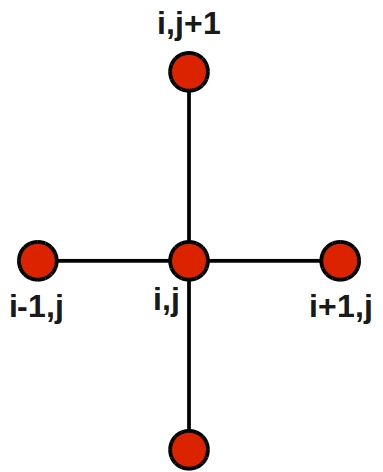
\includegraphics[width=1.5in]{Five-point-stencil.jpg}
\end{center}

The iterative method resulting from our model so far is called the \href{http://en.wikipedia.org/wiki/Carl_Gustav_Jakob_Jacobi}{Jacobi} method. However, please note that this is not a very good method for solving this problem, since if we ``vectorize'' our code then we will get a diagonally dominant matrix that is sparse (i.e. mostly filled with zeros). Therefore, other matrix-based techniques will be more efficient for solving problems modeled with the finite difference method as we will explore later in the course. \\

Below is a Julia function which implements the Jacobi iteration for the 2D steady state heat equation on a $N$ by $N$ grid. The update formula and boundary conditions are as per the previous section (with some minor changes to make the pictures more interesting).\\

\begin{minted}{julia}
#sample call jacobi_heat(120, 100000)

function jacobi_heat(N, maxiter)
    #grid spacing
    h = 1 / (N + 1)
    
    #tolerance
    tolerance = 0.1 / (N+1)^2
    
    #x ad y coordinates of grid points
    x = [0:h:N+1]
    y = [0:h:N+1]
    
    #initialize U
    U = zeros(N+2, N+2)
    
    #top and right boundaries should be initialized to 1
    #U[:, N+2] = ones(N+2)
    #U[N+2, :] = ones(N+2)'
    
    #making the boundary temps more interesting
    for k = 1:N+2
        if 0.3 < x[k] < 0.7
            U[k, N+2] = 1
        end
        
        if 0.3 < y[k] < 0.7  
            U[N+2, k] = 1
        end
    end
    
    iter = 0
    dumax = tolerance
    
    while iter < maxiter && dumax >= tolerance
        Uold = U 
        for j = 2:N+1
            for i = 2:N+1
                U[i,j] = (1/4)*(Uold[i-1,j] + Uold[i+1,j] +
                          Uold[i,j-1] + Uold[i,j+1])
                dumax = max(dumax, abs(U[i,j] - Uold[i,j]))
            end
        end
        iter += 1
    end
    return U
end
\end{minted}

Below is the pseudocolor plot for the resulting matrix $U$.

\begin{center}
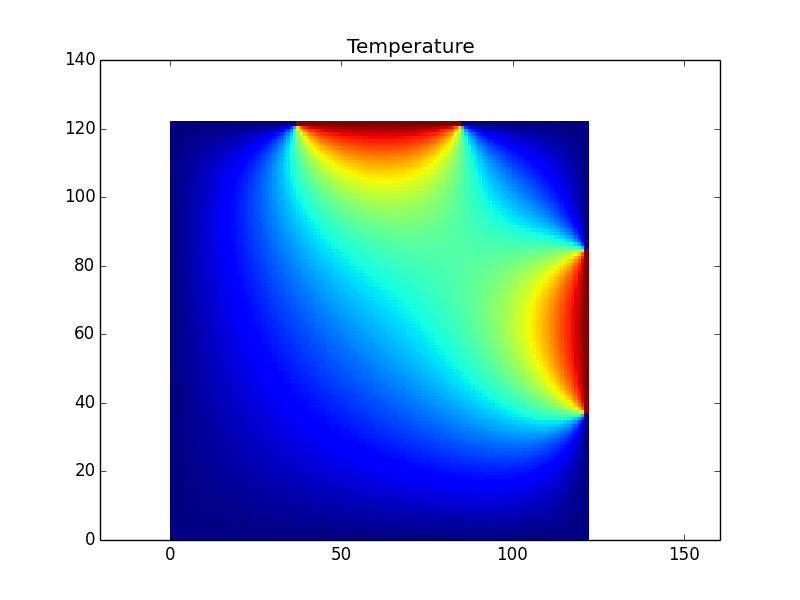
\includegraphics[width=7.25in]{pcolor.png}\\
\end{center}

{\center\color{magenta}
\subsection*{\it\huge Homework 3 (C)}}
\addcontentsline{toc}{subsection}{Homework 3 (C)}
{\it\huge T}here are two components to homework 3 - first there is a conceptual question meant to encourage you to consider historically important PDE's in more detail. The remaining questions are not directly related to PDEs but is instead about benchmarking and performance in Julia, and should both give you further practice with the language as well as a better understanding of its performance characteristics (one of its main advantages relative to other languages oriented towards scientific computing).\\

{\bf Exercises: }
\begin{enumerate}
\item (3 pts each) Choose two of the famous PDE's (e.g. the wave equation, the time-dependent heat equation, etc) listed in the beginning of this lecture. Look up their history and application, and write at least one paragraph about each of them (though more is encouraged) describing what makes them unique and important. You should have at least one source for each PDE you discuss, and you should cite it in \href{http://www.library.cornell.edu/resrch/citmanage/mla}{MLA format}. Commit your work in a file named \verb+hw3PDE.tex+ using appropriate markup (you may find \verb+\footnote{footnote text}+ and \verb+\endnote{endnote text}+ to be useful for citing sources).

\item (2 pts each) In this exercise you will benchmark Julia performance using simple mathematical functions. Your goal is to calculate how many millions of evaluations per second your computer performs for each of the following functions:
\begin{enumerate}
\item An arithmetic operator (addition, subtraction, multiplication, or division)
\item A trigonometric function (sine, cosine, etc.)
\item A logarithm
\item A function you wrote for a previous homework (should take one or two numbers as input, and can return whatever you want as output)
\end{enumerate}

To do this you will want to use either the \verb+@time+ or \verb+@elapsed+ macros. The former prints the time taken to execute but still returns the value from the computation, while the latter directly returns the time elapsed in evaluation instead of the regular return value. \href{http://docs.julialang.org/en/latest/stdlib/base/?highlight=tic#Base.@time}{The Julia manual details these and other related methods.}

To get you started, here is code that draws a million random numbers and then performs a million additions with them, reporting how long it takes for each step:
\begin{verbatim}
N = 1000000
println("rand:  ",  1 / @elapsed x = rand(N))
println("+:     ",  1 / @elapsed x + x)
\end{verbatim}

{\bf Note}: \# of millions operations per second $= 1 \; / $ time elapsed. For instance, if it takes 0.5 seconds to evaluate, then the number of operations per second is $1 / 0.5 = 2$ million.

At a minimum you should execute the benchmark for each operator 10 times, and report the final average. Note that while you could do this manually, it's far wiser to take advantage of the programming language and build a loop around the benchmarking portion, and then sum up and average the overall time. Make sure you report the average of a million operations ran ten times, and not of e.g. ten millions operations run once, as that may be different.

Check in a Julia notebook named \verb+benchmark.ipynb+ that performs the above described benchmarking, as well as a text file \verb+benchmark_output.txt+ that shows your results (both the raw output of running your code, and if necessary further clarification on how many operations per second each operator performs on average).

\item {(1 pt)} Interpret your benchmark results - how did the different functions perform? Why do you think they performed/ranked as they did? Did anything about the results surprise you? Feel free to include your ideas in the \verb+benchmark_output.txt+ file from exercise 2.
\end{enumerate}

%\begin{center}
%\Bart $>$ ``I bet those benchmarks aren't as fast as my skateboard!''
%\end{center}


\newpage
\section*{Lecture 4}
\addcontentsline{toc}{section}{Lecture 4}

{\center\color{magenta}
\subsection*{\it\huge Matrix Algebra}}
\addcontentsline{toc}{subsection}{Matrix Algebra}
Notes coming soon...
{\center\color{magenta}
\subsection*{\it\huge Matrix Operations in Julia}}
\addcontentsline{toc}{subsection}{Matrix Operations in Julia}
Notes coming soon...
\pagebreak

{\center\color{magenta}
\subsection*{\it\huge Homework 4 (P)}}
\addcontentsline{toc}{subsection}{Homework 4 (P)}
{\it\huge T}he purpose of this homework is to have you practice basic linear algebra concepts essential to the understanding of numerical algorithms that require matrix manipulation (which will be introduced later in the quarter). As this homework is to be completed using Julia primarily, it will also serve as practice for writing vectorized code. Complete all of the exercises below in an IJulia notebook using git to add to and revise your work.\\

{\bf Exercises:}
\begin{enumerate}
\item (5 pts)
\begin{enumerate}
\item Consider the following system of linear equations:
\begin{eqnarray*}
2x_1 + x_2 + 5x_3 = -1\\
x_1 + 6x_3 = 2\\
-6x_1 + 2x_2 + 4x_3 = 3
\end{eqnarray*}
On paper, convert this system of equations into a matrix equation of the form {\bf Ax = b} (you do not have to turn this in). In your IJulia notebook, make a comment describing the dimensions of your matrix and vectors. Also explain what it means for us to solve for the vector {\bf x}.
\item Solve for {\bf x}.
\item Using Julia, what is {\bf Ax - b}? Is that what you expected? Explain what you expected and why Julia didn't agree.
\end{enumerate}
\item (5 pts)
\begin{enumerate}
\item Enter the following matrices in Julia:\\
A = 
$\begin{bmatrix}
1 & 2 & 0 \\
2 & 1 & 2 \\
0 & 2 & 1
\end{bmatrix}$, B = 
$\begin{bmatrix}
3 & 0 & 3 \\
1 & 5 & 1 \\
1 & 1 & 3
\end{bmatrix}$, x = 
$\begin{bmatrix}
1\\
2\\
3\\
\end{bmatrix}$

And compute the following expression:
{\bf C} = (2{\bf A}$^2${\bf B} + 3{\bf A}$^T$)$^2$.

\item Now compute the following expressions: {\bf xC}, {\bf Cx} (store this one into a variable {\bf b}), ({\bf Cx})$^T$, and {\bf x}$^T${\bf C}$^T$. Write a few comments explaining the results of each expression and how they compare.

\item Use the built-in \verb+inv+ method to invert the matrix {\bf C}, store it into \verb+Inv_C+. Then compute {\bf Inv\_C*b}. Give a brief mathematical explanation of your result.
\end{enumerate}

\item (5 pts) Suppose we have six cities with airports: Portland, San Francisco, Chicago, New York, Moscow, and Tokyo. We are interested in counting the number of ways we can travel from one city to another with at most $n$ stopovers. \\

Suppose for example that there are direct flights from:
\begin{itemize}
\item Portland to San Francisco;
\item San Francisco to any of the remaining five cities;
\item Chicago to San Francisco, New York, and Moscow;
\item New York to Portland, San Francisco, Chicago, and Moscow;
\item Moscow to Chicago, New York, and Tokyo;
\item Tokyo to San Francisco, New York, and Moscow;
\end{itemize}
and we want to count the number of ways we can get from Portland to Moscow with at most 3 stopovers - e.g., the trip Portland - San Francisco - Tokyo - New York - Moscow is a trip with 3 stopovers. Also, note that for the sake of algorithmic simplicity, we shall include in our count ways that go back and forth between cities - e.g. the trip Portland - San Francisco - Portland - San Francisco - New York is another trip with 3 stop overs.\\

At first glance this problem seems to have little to do with matrices and linear algebra, but it turns out that there is a very easy and elegant way of solving problems of this type using something called an \href{https://en.wikipedia.org/wiki/Incidence_matrix}{incidence matrix}.

The first step is to number our cities in the order they are listed: Portland will be 1, San Francisco will be 2, and so on.  Then, let us set up our incidence matrix {\bf A} by the following rule: if we can get from the $i^{th}$ city to the $j^{th}$ city, then the entry {\bf A}$_{ij}$ of the matrix {\bf A} will be set to 1.  Otherwise we set that entry to 0.  By convention we will set all of the diagonal entries, {\bf A}$_{ii}$ to 0, because you cannot take a flight from a city to itself.  Thus we obtain the following matrix {\bf A} for the given situation:

A = 
$\begin{bmatrix}
0 & 1 & 0 & 0 & 0 & 0 \\
1 & 0 & 1 & 1 & 1 & 1 \\
0 & 1 & 0 & 1 & 1 & 0 \\
1 & 1 & 1 & 0 & 1 & 0 \\
0 & 0 & 1 & 1 & 0 & 1 \\
0 & 1 & 0 & 1 & 1 & 0 
\end{bmatrix}$

\begin{enumerate}
\item Compute {\bf A}$^2$. What is the meaning of {\bf A}$^2$? Write a paragraph or so in your IJulia notebook comments. {\bf Hint: }I recommend performing this computation on paper (in addition to doing it in Julia) and writing all the intermediary steps, in order to better understand its meaning (it will have to do with stopovers).
\item Given the matrix {\bf A} and your insights from part (a) above, solve the original problem of getting from Portland to Moscow with \emph{at most 3} stopovers. Make sure that your solution agrees with your intuition (i.e. get a pencil and paper out and double check your answer). Note, you do not have to worry about eliminating routes that repeat cities, but if you do ... kudos!
\end{enumerate}
\end{enumerate}


\newpage
\section*{Lecture 5 \footnote{Sources for Lecture 5: Chapter 2 from Heath's {\it Scientific Computing: an Introductory Survey} and \href{https://en.wikipedia.org/wiki/System\_of\_linear_equations}{Wikipedia}}}
\addcontentsline{toc}{section}{Lecture 5}

{\center\color{magenta}
\subsection*{\it\huge Solving Systems of Linear Equations}}
\addcontentsline{toc}{subsection}{Solving Systems of Linear Equations}
{\it\huge S}ystems of linear equations are ubiquitous in scientific computing. They can occur naturally, or they can be the result of approximating nonlinear or differential equations from a variety of different fields (we will look at some examples below). Therefore, understanding how such systems are solved and being able to come up with efficient and good solutions for these systems are important skills for computational scientists.\\

A system of linear equations is a collection of equations involving the same set of variables, e.g.
\begin{eqnarray*}
3x_1 + 2x_2 - x_3 = 1\\
2x_1 - 2x_2 + 4x_3 = -2\\
-x_1 + \frac{1}{2}x_2 - x_3 = 0
\end{eqnarray*}

Solving the system above means finding values for $x_1, x_2, x_3$ that satisfy each equation in the system. Note that for a system involving only a few variables (less than 10 or so), such as the one above, we could be persuaded to solve it by hand using the substitution method we've learned in Calculus. However, the more interesting systems will involve hundreds of variables and the above notation, as well as our knowledge of the substitution method, won't scale.\\

We need to model such problems with vector and matrices. Given the definition of matrix-vector multiplication from last week, we can re-write the above system as follows:
\[
\begin{bmatrix}
3 & 2 & -1\\
2 & -2 & 4\\
-1 & \frac{1}{2} & -1
\end{bmatrix}
\begin{bmatrix}
x_1\\
x_2\\
x_3
\end{bmatrix}
=
\begin{bmatrix}
1\\
-2\\
0
\end{bmatrix}
\]

In general, for the system of $m$ linear equations involving $n$ unknowns below:
\begin{eqnarray*}
a_{1,1}x_1 + a_{1,2}x_2 + ... + a_{1,n}x_n = b_1\\
a_{2,1}x_1 + a_{2,2}x_2 + ... + a_{2,n}x_n = b_2\\
\vdots \\
a_{m,1}x_1 + a_{n,2}x_2 + ... + a_{m,n}x_n = b_m\\
\end{eqnarray*}

We have the following matrix equation:
\[
 \begin{bmatrix}
  a_{1,1} & a_{1,2} & \cdots & a_{1,n} \\
  a_{2,1} & a_{2,2} & \cdots & a_{2,n} \\
  \vdots  & \vdots  & \ddots & \vdots  \\
  a_{m,1} & a_{n,2} & \cdots & a_{m,n}
 \end{bmatrix}
 \begin{bmatrix}
 x_1 \\ x_2 \\ \vdots \\ x_n
 \end{bmatrix}
 =
 \begin{bmatrix}
 b_1 \\ b_2 \\ \vdots \\ b_m
 \end{bmatrix}
\] 

If we name the $m \times n$ matrix {\bf A}, the vector of unknowns {\bf x}, and the right-hand side vector {\bf b}. We get the following concise vectorized notation for our linear system: {\bf Ax = b}.\\

Note that the generalized system above allows us to assume that we have a different number of equations than unknowns, however for the sake of introduction we will only consider square systems (i.e. $m=n$) in this lecture.\\ 

\pagebreak
{\it\Large\color{red} Singular Matrices}\\

A square $n \times n$ matrix {\bf A} is singular if the following equivalent properties hold:\\
\begin{enumerate}
\setlength{\itemsep}{0pt}
\item it has no inverse: that is, there does not exist a matrix {\bf M} such that {\bf AM = MA = I} (where {\bf I} is the identity matrix);
\item its determinant is 0. The determinant of a matrix is a special number that tells us interesting things about the solution of a system (kinda like the discriminant tells us interesting things about the solution of a quadratic function). Basically, if the determinant of {\bf A} is 0, then we either have no solution to the system of linear equations or infinitely many solutions;
\item its rank is less than n. The rank of a matrix is the maximum number of linearly independent rows or columns - that is, the maximum number of rows or columns that are not linear combinations (scalar multiples and addition) of other rows or columns in the matrix;
\item {\bf Az = 0} for {\bf z} $\neq$ {\bf 0}, as this basically implies 3 above.\\
\end{enumerate} 

Otherwise, the matrix {\bf A} is said to be \emph{nonsingular}. If that's the case then the inverse of {\bf A}, denoted {\bf A}$^{-1}$, exists and the equation {\bf Ax = b} has the unique solution {\bf x = A}$^{-1}${\bf b}, regardless of the vector {\bf b}. On the other hand, a system of linear equation whose coefficient matrix is singular, may or may not have solutions, and the number of solutions will be determined by the vector {\bf b}.

\begin{framed}
{\bf Example 5.1 } Consider the following system:
\begin{eqnarray*}
2x_1 + 3x_2 = b_1 \\
5x_1 + 4x_2 = b_2
\end{eqnarray*}

We can translate it to vectorized form as follows:
\[
\begin{bmatrix}
2 & 3 \\
5 & 4
\end{bmatrix}
\begin{bmatrix}
x_1 \\
x_2
\end{bmatrix}
=
\begin{bmatrix}
b_1\\
b_2
\end{bmatrix}
\]

Note that \verb+A = [2 3; 5 4]+ (try \verb+det(A)+ in Julia for a quick check) is nonsingular. Thus a unique solution exists and this fact does not depend on the value of the vector {\bf b} (quick exercise: find the unique solution to the system above if \verb+b = [8; 13]+). \\

Now consider the following system:
\begin{eqnarray*}
2x_1 + 3x_2 = b_1 \\
4x_1 + 6x_2 = b_2
\end{eqnarray*}

with vectorized form:
\[
\begin{bmatrix}
2 & 3 \\
4 & 6
\end{bmatrix}
\begin{bmatrix}
x_1 \\
x_2
\end{bmatrix}
=
\begin{bmatrix}
b_1\\
b_2
\end{bmatrix}
\]

Right away we see that the second row of the matrix above has values that are twice the values of the first row for each corresponding value. Thus, whether a solution exists or not will depend on the vector {\bf b}. If, for example {\bf b} = $\begin{bmatrix} 4\\ 7\end{bmatrix}$, then  no solution exists. However, if {\bf b} = $\begin{bmatrix} 4\\ 8\end{bmatrix}$, then {\bf x} = $\begin{bmatrix} \alpha \\ \frac{4 - 2\alpha}{3}\end{bmatrix}$.
\end{framed}

{\bf Note: }Systems of linear equations have intuitive \href{https://en.wikipedia.org/wiki/System_of_linear_equations#Geometric_interpretation}{geometric interpretation}. If we have two unknown variables, the equations are lines on the two dimensional plane. If we have three unknown variables, they are planes in the three dimensional space. And so on...\\

{\it\Large\color{red} Gaussian Elimination}\\

A simple way of solving a system of linear equations that is a bit more algorithmic and efficient than the good old substitution method is via Gaussian elimination of variable. Given a system of linear equations in vectorized for the algorithm sequentially performs elementary row operations on the matrix of coefficients until the lower-left hand corner of the matrix is filled with 0's (as far as possible anyway). The elementary row operations (these are operations that will not change the linear system) are:

\begin{enumerate}
\setlength{\itemsep}{0pt}
\item Exchanging two rows;
\item Multiply a row by a non-zero scalar;
\item Adding a multiple of a row to another row.
\end{enumerate}

Here is a detailed \href{https://en.wikipedia.org/wiki/Gaussian_elimination#Example_of_the_algorithm}{example} of the algorithm being applied to a small linear system. This same technique can be use to compute the determinant of a square matrix or to find the inverse of an invertible (i.e. nonsingular) matrix, amongst other applications.

Here is the pseudocode for the Gaussian elimination algorithm. As an exercise, implement this algorithm in Julia:
\begin{minted}{c}
for k = 1 ... m:
   //Find pivot for column k, that is the index i that maximizes |A[i,k]|:
   i_max  := argmax (i = k ... m, abs(A[i, k]))
   if A[i_max, k] = 0
     error "Matrix is singular!"
   swap rows(k, i_max)
   //Do for all rows below pivot:
    for i = k + 1 ... m:
     //Do for all remaining elements in current row:
      for j = k ... n:
       A[i, j]  := A[i, j] - A[k, j] * (A[i, k] / A[k, k])
     //Fill lower triangular matrix with zeros:
     A[i, k]  := 0
\end{minted}

{\center\color{magenta}
\subsection*{\it\huge Matrix Factorization: LU decomposition}}
\addcontentsline{toc}{subsection}{Matrix Factorization: LU decomposition}
The standard algorithm for solving matrix equations using computers is based on the Gaussian elimination algorithm explained above with some modifications to ensure better efficiency and more accurate results. The commonly used method is called LU decomposition (Lower triangular - Upper triangular decomposition) introduced by Alan Turing.\\

As we've seen in the previous section, applying the Gaussian elimination process to a matrix transforms it into a upper triangular matrix, so that we can easily solve the problem with back-substitution. It can be shown with a bit of theory that there is a matrix {\bf L} such that {\bf A = LU} where {\bf A} is the original matrix of coefficients and {\bf U} is the upper triangular matrix obtained from the Gaussian elimination process.\\

If we can figure out the LU-decomposition for a matrix {\bf A}, then the linear system {\bf Ax = b} can be re-written as {\bf LUx = b}. This system is quick and easy to solve computationally, as we can let {\bf y = Ux} and solve the lower triangular system {\bf Ly = b} via forward-substitution, then the upper triangular system {\bf Ux = y} by back-substitution.

\begin{framed}
{\bf Example 5.2 } Consider the following linear system in three dimensions:
\begin{eqnarray*}
2x_1 +4x_2 - 2x_3 = 2\\
4x_1 + 9x_2 - 3x_3 = 8\\
-2x_1 - 3x_2 + 7x_3 = 10
\end{eqnarray*}
As usual, we can re-write it in matrix notation as such:
\begin{center}
{\bf Ax = }
$
\begin{bmatrix}
2 & 4 &-2\\
4 & 9 &-3\\
-2 &-3 & 7
\end{bmatrix}
\begin{bmatrix}
x_1 \\
x_2 \\
x_3
\end{bmatrix}
=
\begin{bmatrix}
2\\
8\\
10
\end{bmatrix}
$
{\bf = b}.
\end{center}
We can perform Gaussian elimination by subtracting two times the first row from the second row, and adding the first row to the third row - this will eliminate the sub-diagonal entries in first column. Then, we subtract the second row from the third row  - this will eliminate the sub-diagonal entry in second column.\\

This series of operations can be represented by the following matrix multiplication:
\[
\begin{bmatrix}
1 & 0 & 0\\
0 & 1 & 0\\
0 & -1 & 1
\end{bmatrix}
\cdot
\begin{bmatrix}
1 & 0 & 0\\
-2 & 1 & 0\\
1 & 0 & 1
\end{bmatrix}
\cdot
\begin{bmatrix}
2 & 4 &-2\\
4 & 9 &-3\\
-2 &-3 & 7
\end{bmatrix}
=
\begin{bmatrix}
2 & 4 &-2\\
0 & 1 & 1\\
0 & 0 & 4
\end{bmatrix}
=U
\]
The result is an upper triangular matrix which we will call {\bf U}. Since we want to find two matrices {\bf L} and {\bf U}, such that {\bf A= LU}, then given the above matrix multiplication we conclude that {\bf L} is the following lower triangular matrix:
\[
\left(
\begin{bmatrix}
1 & 0 & 0\\
0 & 1 & 0\\
0 & -1 & 1
\end{bmatrix}
\cdot
\begin{bmatrix}
1 & 0 & 0\\
-2 & 1 & 0\\
1 & 0 & 1
\end{bmatrix}
\right)^{-1} =
\begin{bmatrix}
1 & 0 & 0\\
2 & 1 & 0\\
-1 & 0 & 1
\end{bmatrix}
\cdot
\begin{bmatrix}
1 & 0 & 0\\
0 & 1 & 0\\
0 & 1 & 1
\end{bmatrix}
= 
\begin{bmatrix}
1 & 0 & 0\\
2 & 1 & 0\\
-1 & 1 & 1
\end{bmatrix}
\]

{\small (for more information on why the above equality makes sense, please read this \href{http://math.mit.edu/linearalgebra/ila0205.pdf}{chapter} from Strang's Linear Algebra textbook)}\\

Now set {\bf Ux = y}, then we can easily solve for {\bf y} in the system {\bf Ly = b} using forward-substitution:
\[
\begin{bmatrix}
1 & 0 & 0\\
2 & 1 & 0\\
-1 & 1 & 1
\end{bmatrix}
\begin{bmatrix}
y_1 \\
y_2 \\
y_3
\end{bmatrix}
=
\begin{bmatrix}
2\\
8\\
10
\end{bmatrix}
\]

$\Rightarrow y_1 = 2$, $y_2 = 4$ and $y_3 = 8$. Now we use back-substitution to solve for {\bf x} in the system {\bf Ux = y}:
\[
\begin{bmatrix}
2 & 4 & -2\\
0 & 1 & 1\\
0 & 0 & 4
\end{bmatrix}
\begin{bmatrix}
x_1 \\
x_2 \\
x_3
\end{bmatrix}
=
\begin{bmatrix}
2\\
4\\
8
\end{bmatrix}
\]
$\Rightarrow x_3 = 2$, $x_2 = 2$ and $x_1 = -1$, so we get the solution {\bf x = } $\begin{bmatrix}-1\\2\\2\end{bmatrix}$.
\end{framed}
\pagebreak

{\center\color{magenta}
\subsection*{\it\huge Homework 5 (C)}}
\addcontentsline{toc}{subsection}{Homework 5 (C)}
{\it\huge T}he purpose of this homework is to further improve your understanding of how the LU decomposition of a matrix {\bf A} can be used to quickly and easily solve the matrix equation {\bf Ax = b}. You will also gain a bit of historical knowledge on Gaussian elimination, as well as be introduced to the idea of pivot elements for obtaining more accurate results when performing Gaussian elimination computationally.\\

{\bf Exercises: }\\

\begin{enumerate}
\item (5 pts) Write a Julia function that takes as input the matrices {\bf L}  and {\bf U} (from the LU-decomposition of some matrix {\bf A}) and a vector {\bf b}, and outputs the solution vector {\bf x} from the matrix equation {\bf Ax = b}. You algorithm should mimic example 5.2 above in that it should perform forward-substitution followed by back substitution appropriately. Then compare your result with \verb+A\b+.
\item (5 pts) Read this \href{http://www.ams.org/notices/201106/rtx110600782p.pdf}{paper} and write a two page summary using \LaTeX.
\item (5 pts) Read this \href{http://college.cengage.com/mathematics/larson/elementary_linear/4e/shared/downloads/c10s1.pdf}{chapter} and answer the following questions (your answers should be typeset):
\begin{enumerate}
\item What is a pivot element for a matrix?
\item Why is it important to use pivoting when performing Gaussian elimination?
\item Solve exercise 22 on page 541 as described there.\\
\end{enumerate}
\end{enumerate}

{\it Commit and push your .ipynb, .tex, and .pdf files for this homework into your GitHub private repository by 5/12 at 11:59 PM.}

\newpage
\section*{Lecture 6}
\addcontentsline{toc}{section}{Lecture 6}

{\center\color{magenta}
\subsection*{\it\huge Linear Regression with One Variable}}
\addcontentsline{toc}{subsection}{Linear Regression with One Variable}

{\it\huge L}inear regression is a statistical learning approach for quantitatively predicting an outcome {\bf y} on the basis of predictor variables {\bf x}$_j$, such that the relationship between the outcome and the variables is linear. Mathematically we write
\[
\textnormal{{\bf y}} \approx  \theta_0 +
\theta_1 \textnormal{{\bf x}}_1 +
\theta_2 \textnormal{{\bf x}}_2 + ... +
\theta_n \textnormal{{\bf x}}_n
\]

that is {\bf y} can be approximated by a linear combination of $n$ predictor variables.\\

In this lecture we will focus our attention on single variable regression and leave the multivariable case for the next lecture. In the single variable case we have that the outcome {\bf y} can be approximated by a linear relationship involving only one variable {\bf x}, or mathematically
\[
\textnormal{{\bf y}} \approx  \theta_0 +
\theta_1 \textnormal{{\bf x}}
\]

{\it\Large\color{red} Supervised Learning}\\

There are different contexts in which we may discuss the topic of linear regression. In this lecture, we will study it in the light of machine learning and thus use vocabulary pertinent to this field. In machine learning there are two main sorts of problems: supervised learning and unsupervised learning problems. In this course we will only address supervised learning problems. \\

In supervised learning, we wish to infer a function that classifies or fits future data, based on a training data set (that is, data that we already have collected and know the ``right'' output for each input). Let us motivate our discussion with an example. Consider the following training data set below, where we have on the left column the number of years for which a person went to school and on the right column the income they now make, in thousands of dollars per year.\\

\begin{verbatim}
"Education"    "Income"
 10.0           26.6588   
 10.4013        27.3064   
 10.8428        22.1324   
 11.2441        21.1698   
 11.6455        15.1926   
 12.087         26.399    
 12.4883        17.4353   
 12.8896        25.5079   
 13.291         36.8846   
 13.7324        39.6661   
 14.1338        34.3963   
 14.5351        41.498                    
\end{verbatim}  
$\vdots$

Here our ``$x$'' or input is the education level of an individual, while our ``$y$'' or output is the income level of the same individual. Since we have many inputs for different observations (say $m$ of them), then we put them all in a $m \times 1$ vector {\bf x}. Similarly, {\bf y} is a $m \times 1$ vector of outputs. In linear regression, we wish to infer the function of the line that best fits data in a certain input-output relationship, that is, we wish to come up with a linear function
\[
\textnormal{{\bf h$_{\theta}$(x)}} =  \theta_0 +
\theta_1 \textnormal{{\bf x}}
\]
 that best approximates our output vector {\bf y}.
 
In the formula above we have that $\theta_j$'s are the parameters or the weights of the linear map from {\bf x} to {\bf y}. So we want to find the parameters (in this case they are the slope and $y$-intercept of our line) that give us a line of best fit:
\begin{center}
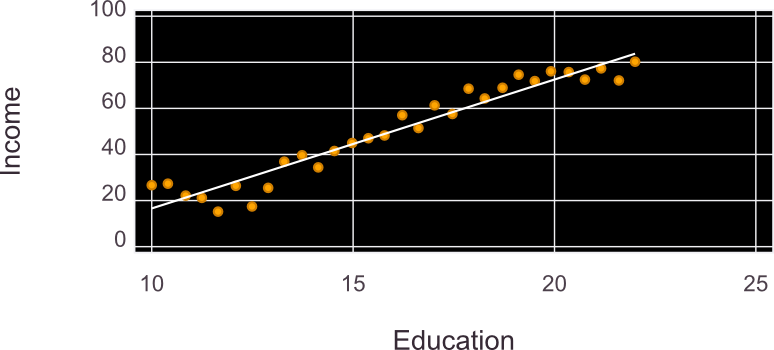
\includegraphics[scale=1.3]{myplot.png}
\end{center}

So how do we choose the parameters $\theta_j$? In this lecture we will do that via the Gradient Descent Method. In the next lecture we will generalize linear regression and gradient descent for multiple variables (that is, multiple input vectors {\bf x}$_j$), and learn yet another technique we can use for solving for the parameters $\theta_j$. But before we get into all that, let us get a better intuition for these parameters, simply by experimenting with a few different combinations of $\theta_0$ and $\theta_1$:\\

\begin{minipage}{2in}
{\small $h(x) = \theta_0 + \theta_1 x$, \\
$\theta_0 = 1.5, \theta_1 = 0$:\\}
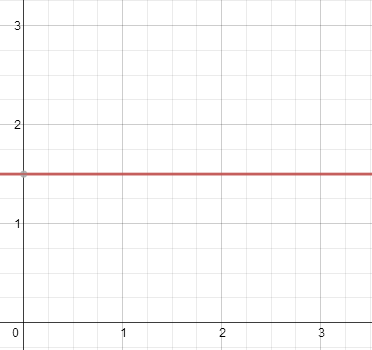
\includegraphics[width=1.5in]{plot1.png}
\end{minipage}
\begin{minipage}{2in}
{\small $h(x) = \theta_0 + \theta_1 x$, \\
$\theta_0 = 0, \theta_1 = 0.5$:\\}
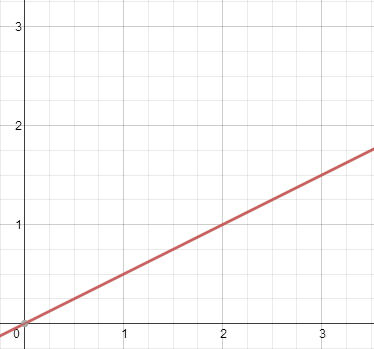
\includegraphics[width=1.5in]{plot2.png}
\end{minipage}
\begin{minipage}{2in}
{\small $h(x) = \theta_0 + \theta_1 x$, \\
$\theta_0 = 1, \theta_1 = 0.5$:\\}
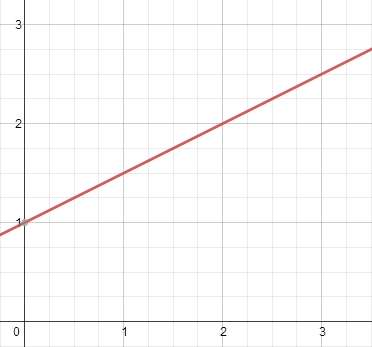
\includegraphics[width=1.5in]{plot3.png}\\
\end{minipage}

Note how changing the parameters $\theta_j$ changes the slope and position of our line in the plane. As an exercise, I encourage students to read different data sets in julia (with one input variable, where the output is quantitative), scatter plot the data and play around with manually picking the slope and intercept parameters for the line that best fits the data visually.\\

{\it\Large\color{red} The Cost Function}\\

In order for us to be able to apply the gradient descent algorithm for solving our liner regression problem, we will need a function to minimize (as we will see later gradient descent is an algorithm for finding the input that minimizes the output value of a function). This function is called the cost function and it is defined as follows:
\[
C(\theta_0, \theta_1) = \frac{1}{2m}\sum\limits_{i=1}^m(h_{\theta} (x^{(i)}) - y^{(i)})^2
\]

This function outputs the sum of the squared errors between the predicted outputs and the actual outputs, given inputs $\theta_0$ and $\theta_1$. Thus, minimizing this function means getting the $\theta_0$ and $\theta_1$ that causes $C$ to be smallest. It seems intuitive to minimize the magnitude of the errors, but you may be wondering why minimize the squared errors versus just the absolute value of the errors. For our purposes, the explanation is simple - minimization means taking derivatives, and therefore the cost function must be continuous and differentiable. Also, \href{https://en.wikipedia.org/wiki/Carl_Friedrich_Gauss}{Gauss} proved that minimizing the cost function $C$ defined above (aka the ordinary least squares method) gives the \href{http://en.wikipedia.org/wiki/Gauss%E2%80%93Markov_theorem}{best} estimate to the linear regression problem.\\

Note that the cost function is a multivariate quadratic function. If $C$ were a quadratic function of one variable, then in a two dimensional space its graph would look like a concave-up parabola. Such a parabola would have a global minimum at the vertex. Analogously, in our case $C$'s graph lives in a three dimensional space and it is a ``bowl-up'' shaped surface, with a global minimum at the base of the bowl.\\

\begin{center}
{\bf The surface plot: }\\
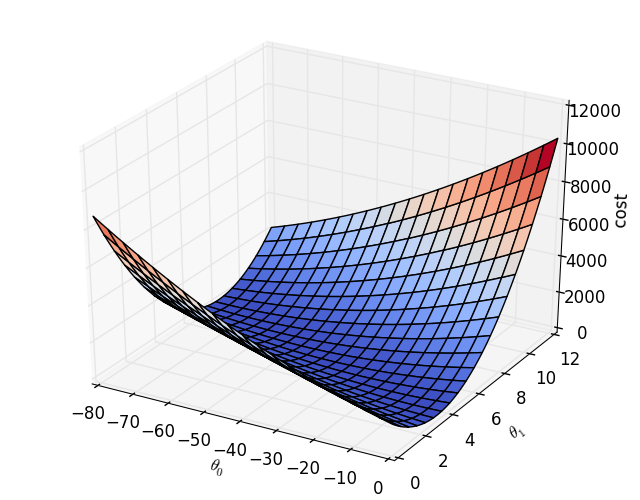
\includegraphics[scale=.6]{cost.png}\\
\end{center}
\vspace{1in}
\begin{center}
{\bf The contour plot: }\\
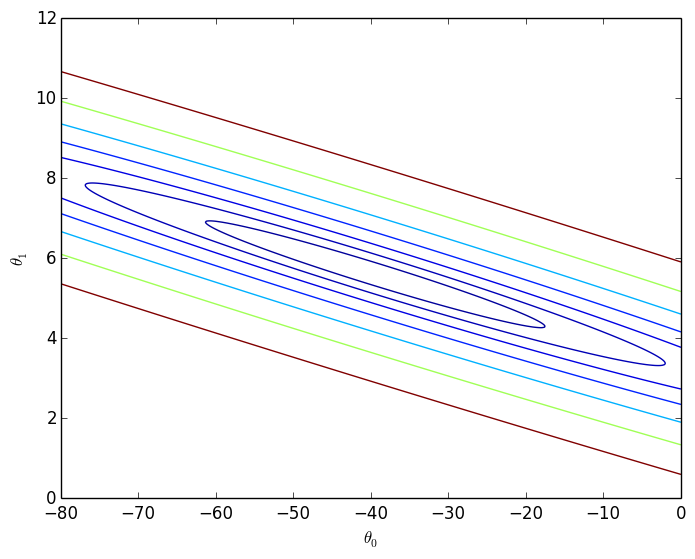
\includegraphics[scale=.5]{costContour.png}
\end{center}
\newpage

{\center\color{magenta}
\subsection*{\it\huge Gradient Descent}}
\addcontentsline{toc}{subsection}{Gradient Descent}

{\it\huge I}n this section we will explore the gradient descent algorithm for optimizing the cost function defined earlier. If you are familiar with Newton's algorithm for finding the roots of a function, you may view the gradient descent algorithm as a generalization of Newton's algorithm. The gradient descent algorithm is a type of search algorithm, that is we start with an initial guess and then we update our guess iteratively by some rule. The rule for gradient descent is that from our previous guess we should step down (with some step size) toward the direction of steepest descent. If we iterate this rule in a ``bowl-up'' shaped surface with a not-to-large step size, we shall converge to a minimum.

\begin{framed}
{\bf Gradient Descent Algorithm for Bivariate Functions}\\

\noindent repeat until convergence \{\\
\indent for $j = 0$ and $j = 1$, simultaneously update:
\[
\theta_j := \theta_j - \alpha \frac{\partial}{\partial \theta_j} C(\theta_0,\theta_1)
\]
\}

\end{framed}
So we take a guess on each $\theta$, then update each $\theta$ simultaneously by taking a step of size $\alpha$ in the respective direction of steepest descent as dictated by the partial derivative of the cost function with respect to the $\theta$ that is being updated. The intuition here is that the slope of the tangent line to our current point is the steepest slope we can get on a line that would still include the point.\\

In machine learning, we call the $\alpha$ parameter ``the learning rate''. An important note is that if $\alpha$ is too large our algorithm may diverge, as our steps will be so large as to ``climb the walls'' of our surface. On the other hand, if $\alpha$ is too small, our algorithm may take a long time to converge. Tweaking $\alpha$ can be seen as more of an art than a science and it will depend on your particular problem. The best way to check that you are picking a good $\alpha$ is to graph (or otherwise output) your cost and verify that it is indeed decreasing and the rate of decrease is not too slow.\\

Using basic Calculus you can easily verify that:
\[
j = 0 \Rightarrow \frac{\partial}{\partial \theta_0}C(\theta_0,\theta_1) = \frac{1}{m}\sum\limits_{i=1}^m(h_{\theta}(x^{(i)})-y^{(i)})
\]

\[
j = 1 \Rightarrow \frac{\partial}{\partial \theta_1}C(\theta_0,\theta_1) = \frac{1}{m}\sum\limits_{i=1}^m(h_{\theta}(x^{(i)})-y^{(i)})\cdot x^{(i)}
\]

\begin{center}
\line(1,0){250}
\end{center}

So now we have a powerful tool for determining the $\theta$ parameters in your linear regression model. Please see the accompanying IJulia notebook illustrating linear regression applied to the education versus income data for more details. \\
\newpage

{\center\color{magenta}
\subsection*{\it\huge Homework 6 (P)}}
\addcontentsline{toc}{subsection}{Homework 6 (P)}

{\it\huge T}he purpose of this homework is to have you practice the method of ordinary least squares and the gradient descent algorithm for solving a linear regression problem. For best results completing this homework, please review the ``Lecture 6'' notes above and the IJulia notebook containing a detail example of linear regression.\\

{\bf Exercises:}\\

The Advertising data set (found in ``Advertising.csv'' on Canvas or GitHub) has data pertaining to the sales in thousands of units versus the advertising budget in thousands of dollars of different advertising media such as TV, radio and newspaper.\\
\begin{enumerate}
\item (9 pts) Using linear regression with least squares and gradient descent, as outlined in lecture 6,  determine the line that best fits the relationship between sales and advertising budget for each medium.
\item (2 pts) Plot your solution line against the data for each feature considered (that is, sales versus TV budget, radio budget and newspaper budget).
\item (2 pts) Plot the surface of your cost function for each feature considered.
\item (2 pts) Compare your results. Is there a medium for advertising that you would claim to be best above all others? Which one and why? Write a short report of your findings using \LaTeX. Make sure to include your formulas and figures obtained in the process of solving this problem.
\end{enumerate}

{\it Commit and push your .ipynb, .tex, and .pdf files for this homework into your GitHub private repository by 5/19 at 11:59 PM.}

\newpage
\section*{Lecture 7\footnote{Source for Lecture 7: Stanford's Machine Learning \href{http://cs229.stanford.edu/notes/cs229-notes1.pdf}{Lecture Notes}}}
\addcontentsline{toc}{section}{Lecture 7}

{\center\color{magenta}
\subsection*{\it\huge Linear Regression with Multiple Variables}}
\addcontentsline{toc}{subsection}{Linear Regression with Multiple Variables}

{\it\huge T}his lecture will continue our discussion of linear regression, the statistical learning approach for quantitatively predicting an outcome {\bf y} on the basis of predictor variables {\bf x}$_j$. We have already studied in depth the single variable regression problem, now we will explore linear regression with multiple variables (or features, as per our machine learning vocabulary):
\[
\textnormal{{\bf y}} \approx  \theta_0 +
\theta_1 \textnormal{{\bf x}}_1 +
\theta_2 \textnormal{{\bf x}}_2 + ... +
\theta_n \textnormal{{\bf x}}_n
\]

that is {\bf y} can be approximated by a linear combination of $n$ predictor variables.\\

As an example we will consider the advertising training data set from homework 6, but instead of looking at how each feature affects sales individually, we will look at how they do so combined. Recall that sales is in thousands of units, and the different media advertising budgets are in thousands of dollars.\\

\begin{verbatim}
In [1]: ad = readcsv("Advertising.csv")

Out[1]:
201x4 Array{Any,2}:
    "TV"    "Radio"    "Newspaper"    "Sales"
 230.1    37.8       69.2           22.1     
  44.5    39.3       45.1           10.4     
  17.2    45.9       69.3            9.3     
 151.5    41.3       58.5           18.5     
 180.8    10.8       58.4           12.9     
   8.7    48.9       75.0            7.2     
  57.5    32.8       23.5           11.8     
 120.2    19.6       11.6           13.2     
   8.6     2.1        1.0            4.8     
 199.8     2.6       21.2           10.6     
  66.1     5.8       24.2            8.6     
 214.7    24.0        4.0           17.4     
\end{verbatim}  
$\vdots$\\
                                                            
Here our ``$x$'' values (or inputs, or features) are the different media advertising budgets - each row is an advertising campaign, while our ``$y$'' (or output) is the total number of units sold as a result of each of the advertising campaigns. Since we have many advertising campaigns (say $m$ of them) with three features, then we put them all in a $m \times 3$ matrix {\bf X}. Similarly, {\bf y} is a $m \times 1$ vector of outputs. As before, we wish to infer the function of the ``line'' (in this case a three-dimensional plane) that best fits data in a certain input-output relationship, that is, we wish to come up with a multivariate linear function
\[
\textnormal{{\bf h$_{\theta}$(x)}} = \theta_0 +
\theta_1 \textnormal{{\bf x}}_1 +
\theta_2 \textnormal{{\bf x}}_2 + ... +
\theta_n \textnormal{{\bf x}}_n
\]
 that best approximates our output vector {\bf y}.\\
 
In the formula above we have that $\theta_j$'s are the parameters or the weights of the linear map from {\bf X} to {\bf y}. Since we will want to vectorize our code for convenience, we add a column of ones in front of the matrix {\bf X} to account for the $\theta_0$ parameter, as such \verb+X = [ones(m,1) X]+.\\

For the sake of showing a picture, here is the scatter plot for sales (on the $z$-axis) versus the advertisement budgets for TV and radio:
\begin{center}
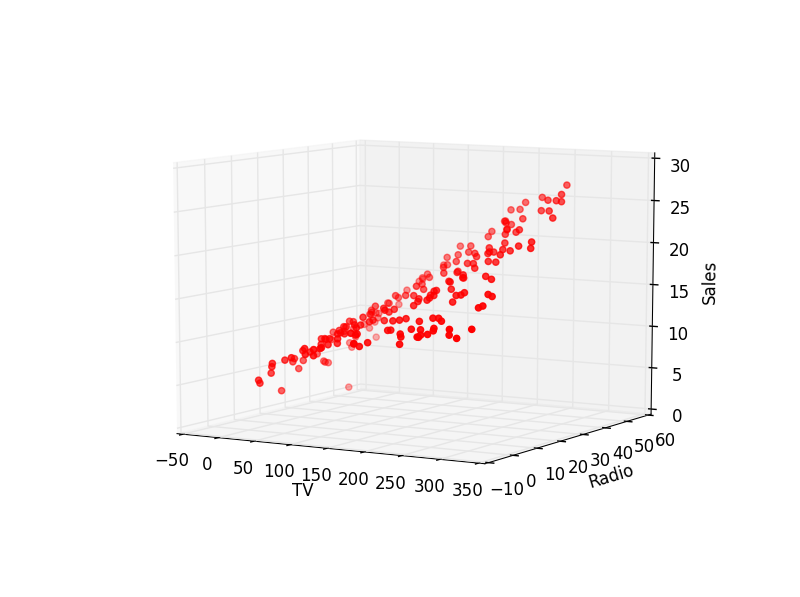
\includegraphics[scale=.5]{scatter3d.png}
\end{center}

If the TV and Radio budgets were the only features in our advertising model, then the goal of linear regression would be for use to fit a two dimensional plane such that the squared errors are minimized, just as in the single variable case. So we can see that the ideas we learned last week can be generalized to multiple variable. The down side of having more than two features, however, is that we will have a hard time graphing our data! We can try some cleaver tricks (such as having TV, Radio and Newspaper on the x, y, and z axis respectively, while sales is represented by the size of the circles...), but at the end of the day we need to rely on our numbers.
\begin{center}
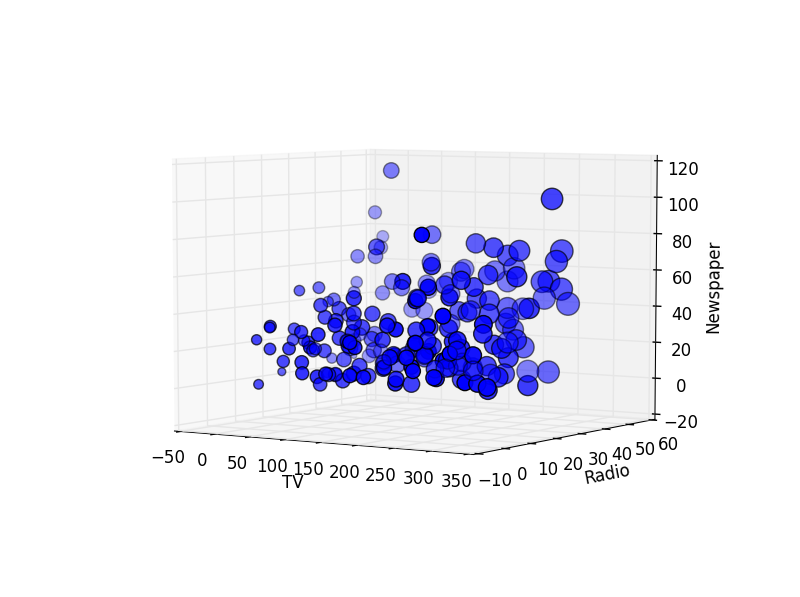
\includegraphics[scale=.5]{scatter4d.png}
\end{center}

In this lecture we will continue to explore the method of \emph{gradient descent} to find the parameters $\theta_j$. We will also learn about the \emph{normal equation} method, an analytic way for exactly solving for the parameters $\theta_j$, which works well if your data is not too large.\\

For using the gradient descent method we will still need the \emph{cost function}, which will remain mostly the same as before. The only difference will be {\bf h$_{\theta}$(x)} (recall here that each feature {\bf x}$_j$ is a $m \times 1$ vector representing different observed values):

\[
\textnormal{{\bf h$_{\theta}$(x)}} = \theta_0 +
\theta_1 \textnormal{{\bf x}}_1 +
\theta_2 \textnormal{{\bf x}}_2 + ... +
\theta_n \textnormal{{\bf x}}_n
\]

If we define {\bf x}$_0$ = \verb+ones(m,1)+, that is a vector of $m$ ones, then we can rewrite {\bf h$_{\theta}$(x)} as such:
\[
\textnormal{{\bf h$_{\theta}$(x)}} = 
\theta_0 \textnormal{{\bf x}}_0 +
\theta_1 \textnormal{{\bf x}}_1 +
\theta_2 \textnormal{{\bf x}}_2 + ... +
\theta_n \textnormal{{\bf x}}_n
= \textnormal{{\bf X$\theta$}}
\]

where {\bf X} is the $m \times n$ matrix $\begin{bmatrix}
| & | & & |\\
\textnormal{{\bf x}}_0 & \textnormal{{\bf x}}_1 & \hdots & \textnormal{{\bf x}}_n\\
| & | & & |
\end{bmatrix}$, while $\theta$ is the $n \times 1$ column vector $\begin{bmatrix}
\theta_0\\
\theta_1\\
\vdots\\
\theta_n
\end{bmatrix}$.

Thus our ``new'' cost function looks a lot like the old one, however it's input now is the $n \times 1$ column vector $\theta$:
\[
C(\theta) = \frac{1}{2m}\sum\limits_{i=1}^m(h_{\theta} (x^{(i)}) - y^{(i)})^2
\]

{\center\color{magenta}
\subsection*{\it\huge Gradient Descent for Multiple Variables}}
\addcontentsline{toc}{subsection}{Gradient Descent for Multiple Variables}

Since the cost function did not change too dramatically, the gradient descent recipe will also only change slightly:

\begin{framed}
{\bf Gradient Descent Algorithm}\\

\noindent repeat until $C$ converges to a minimum \{\\
\indent for $j = 0,1,...,n$, simultaneously update:
\[
\theta_j := \theta_j - \alpha \frac{\partial}{\partial \theta_j} C(\theta)
\]
\}\\

where

\[
\frac{\partial}{\partial \theta_j}C(\theta) = \frac{1}{m}\sum\limits_{i=1}^m(h_{\theta}(x^{(i)})-y^{(i)})\cdot x^{(i)}
\]

\end{framed}


And the interpretation is still the same as before: we take a guess on each $\theta$, then update each $\theta$ simultaneously by taking a step of size $\alpha$ in the respective direction of steepest descent as dictated by the partial derivative of the cost function with respect to the $\theta$ that is being updated.\\


{\center\color{magenta}
\subsection*{\it\huge Good Practice: Feature Scaling}}
\addcontentsline{toc}{subsection}{Good Practice: Feature Scaling}

A good practice technique that becomes important when we have more than one feature in our model is called \emph{feature scaling}. The idea here is that most of the time we have features that are on widely different ranges and scales from each other. For example, if we want to predict housing prices in Seattle, we might want to use the size of the house in square feet as a feature (say {\bf x}$_1$) and the number of bedrooms as another (say {\bf x}$_2$). So the values in {\bf x}$_1$ will range from 300 to 3000, while the values in {\bf x}$_2$ will range from 0 to 5.\\

You can imagine that his will cause the graph of our cost function to be narrow along the $\theta_1$ dimension and wide along the $\theta_2$ dimension. Thus, depending on where your initial $\theta$ finds itself, the gradient descent algorithm may take much longer to converge to the minimum value of $C(\theta)$, and in this case increasing $\alpha$ may not help (and may even cause a quicker divergence). \\

{\it\Large\color{red} Mean Normalization and Scaling}\\

There are different ways to fix the problem above. The idea in all of them is to make all of our features have values that lie in the same range roughly from -1 to 1 (times 2 or 3 is also ok). A preferred technique is \emph{mean normalization} with standard deviation scaling, that is for each value $x^{(i)}$ in each feature vector {\bf x}$_j$, replace is with:

\[ \frac{x^{(i)} - \mu_j}{\sigma_j} \]

where $\mu_j$ is the mean value of the values in {\bf x}$_j$, and $\sigma_j$ is the standard deviation of the values in {\bf x}$_j$. Another common practice would be to scale with the size of the range of values in a particular feature vector (i.e. max - min) instead of the standard deviation.\\

And as before, the best way to check that your feature scaling is working and that you are picking a good $\alpha$ is to graph (or otherwise output) your cost versus the number of gradient descent iterations and verify that the cost is indeed decreasing and the rate of decrease is not too slow at each iteration.\\

{\center\color{magenta}
\subsection*{\it\huge The Normal Equation}}
\addcontentsline{toc}{subsection}{The Normal Equation}

\[ A^TAx = A^Tb \]

So far we've been using the gradient descent method for performing linear regression on pretty small problems (gradient descent is meant for big problems, i.e. 10000 features or so). This is because we could not solve the matrix equation {\bf Ax = b} with the ideas learned from lectures 4 and 5, since {\bf A} is usually not square and we cannot invert non-square matrices.\\

The mathematical trick here is: multiply both sides of the matrix equation {\bf Ax = b} on the left by {\bf A}$^T$. Thus we get the normal equation above and it turns out that the solution to the normal equation, that is,
\[ x = (A^TA)^{-1}A^Tb \]

is the \emph{least-squares} solution to the original system of linear equation represented by {\bf Ax = b} (i.e. the solution to the normal equation minimizes the sum of squared errors {\bf b - Ax}). I will not go over the mathematical reason why the normal equation works, as that is beyond the scope of this course, but \href{http://math.mit.edu/linearalgebra/ila0403.pdf}{here} is a resource for further exploration.\\

Given your expertise with matrices by now, you may be wondering what if {\bf A}$^T${\bf A} is singular? Then we cannot find the inverse. That is true...so we find the \href{https://en.wikipedia.org/wiki/Moore%E2%80%93Penrose_pseudoinverse}{pseudoinverse} (in julia we use the \verb+pinv+ function).\\ 

{\it For more details on linear regression with multiple variables and the normal equation method for solving non-square linear systems, please see the accompanying IJulia notebook.}\\

\pagebreak

{\center\color{magenta}
\subsection*{\it\huge Homework 7 (C)}}
\addcontentsline{toc}{subsection}{Homework 7 (C)}

{\it\huge T}he purpose of this homework is to ensure your conceptual understanding of the topics presented in lecture 7. Please typeset your \emph{complete solution} to each exercise below using \LaTeX.\\

{\bf Exercises:}\\
\begin{enumerate}
\item (3 pts) Suppose $m=4$ students have taken some class, and the class had two midterm exams and a final exam. You have collected a data set of their scores on the three exams, which is as follows:
\begin{center}
\begin{tabular}{| c | c | c |}
\hline
midterm 1 & midterm 2 & final exam\\
\hline
89 & 91 & 96 \\
\hline
72 & 77 & 74 \\
\hline
94 & 90 & 87 \\
\hline
69 & 70 & 78 \\
\hline
\end{tabular}
\end{center}
You'd like to use linear regression to predict a student's final exam score from their midterm exams scores. Concretely, suppose you want to fit a model of the form {\bf h$_{\theta}$(x)= $\theta_0$ + $\theta_1$x$_1$ + $\theta_2$x$_2$}, where {\bf x}$_j$ is the vector of midterm $j$ scores. Further, you plan mean normalization and scale the features using the size of the range of values. What is the normalized feature $x^{(1)}_1$? (Recall that the superscript indicates the particular observation, while the subscript indicates the particular feature). Please show your work.
\item (3 pts) You run gradient descent for 15 iterations with $\alpha=0.3$ and compute $C(\theta)$ after each iteration. You find that the value of $C(\theta)$ decreases slowly and is still decreasing after 15 iterations. Based on this, what is your conclusion and course of action?
\item (3 pts) Why should we perform feature scaling?
\item (3 pts) Suppose you have a data set with $m=50$ examples and $n=15$ features for each example. You want to use multivariate linear regression to fit the parameters $\theta$ to your data. Should you prefer gradient descent or the normal equation? Why?

\item (3 pts) Find the least-squares solution of the matrix equation {\bf Ax = b} (for the given {\bf A} and {\bf b} below) using the normal equation {\bf A}$^T${\bf Ax = A}$^T${\bf b}. You should show your work step by step. Including images or skipping steps is allowed, but typesetting it \emph{completely} using \LaTeX $\;$ is worth +2 points.
\[
\textnormal{A} = \begin{bmatrix}
1 & -2\\
-1 & 2\\
0 & 3 \\
2 & 5
\end{bmatrix}
\;\;\;
\textnormal{b} = \begin{bmatrix}
3 \\ 1 \\ -4 \\ 2
\end{bmatrix} 
\]
\end{enumerate}

{\it Commit and push your .tex, {\bf and} .pdf files for this homework into your GitHub private repository by 5/26 at 11:59 PM.}


\newpage


\section*{Lecture 8}
\addcontentsline{toc}{section}{Lecture 8}

{\center\color{magenta}
\subsection*{\it\huge Logistic Regression}}
\addcontentsline{toc}{subsection}{Logistic Regression}

{\it\huge L}ast week we learned about linear regression, where our goal was to predict a quantitative outcome {\bf y} given a linear relationship between multiple inputs {\bf x}$_j$. However for many different problems, when given an observation, we may wish to make a qualitative prediction instead. For example, we may wish to determine whether or not a patient has a high cancer risk or whether or not an email is spam. In this lecture we will study logistic regression, an approach used in statistics and machine learning for predicting qualitative outcomes. \\

In machine learning, this sort of approach is more commonly known as \emph{classification}, due to the fact that we seek to assign our observations (or training examples) to a category or class, thus classifying them. So now our outcome {\bf y} is a vector of categories or classes. Here, since we will be studying logistic regression, we will consider two classes for the outcomes: 0 or the ``negative'' class (e.g. not high cancer risk, not spam); and 1 or the ``positive'' class (e.g. high cancer risk, spam). \\

Please note that there are other approaches than logistic regression for classifying data. Also note that there are other approaches and techniques that would accommodate predicting for more than two classes. We will briefly address the approach of applying logistic regression many times in order to classify data into more than two categories, however a deeper study of different classification techniques is left to the reader. At the end of this lecture, I will provide resources for further study of classification.\\

The first question we should ask ourselves is: why do we need a different technique than linear regression? Can't we just apply linear regression and if the outcome for an observation is below 0.5 we predict ``negative'', otherwise we predict ``positive''? \\

\begin{center}
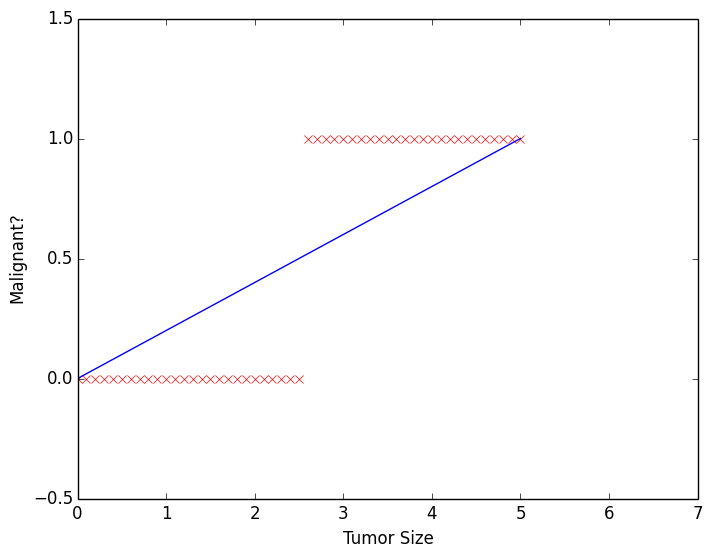
\includegraphics[width=4.5in]{logregexample.png}\\
\end{center}
\newpage

Well, let's think about how an outlier can change our predictions if we were to use linear regression:\\

\begin{center}
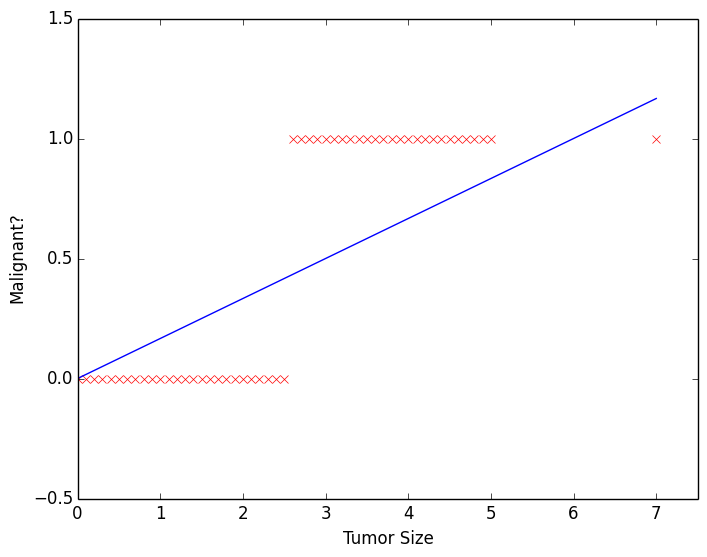
\includegraphics[width=4.5in]{logregexample2.png}\\
\end{center}

In the above picture, this outlier will change the slope of our line of best fit and cause us to classify several positive cases as negative. Therefore, it looks like we cannot rely on linear regression alone to help us classify data. It turns out there is a function in which we can plug in the result of our linear regression in order to get a discretezation of categories that will not be affected by outliers - this function is called the \emph{sigmoid}:

\[
\textnormal{sigmoid}(z) = \frac{1}{1+e^{-z}}
\]

Here is its graph:

\begin{center}
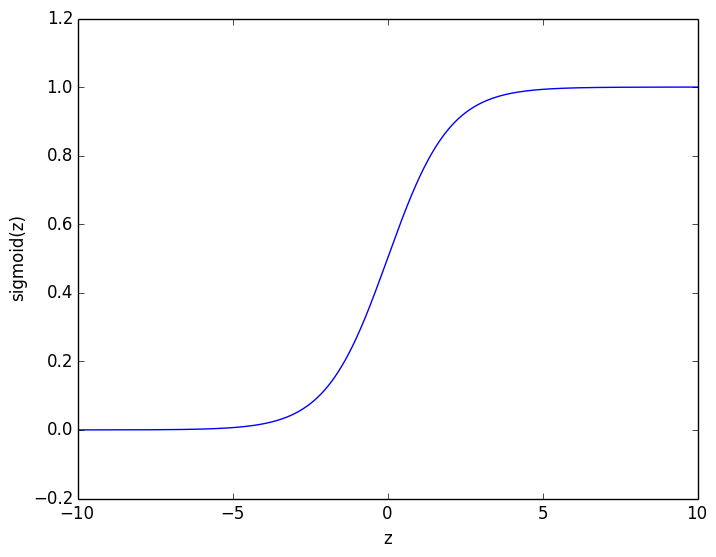
\includegraphics[width=4.5in]{sigmoid.png}\\
\end{center}

Thus, in our attempt to find a {\bf h$_{\theta}$}({\bf x}) that best approximates the true observed outcome {\bf y} (as we did with linear regression), if we were to interpret $h_{\theta}(x^{(i)})$ as the estimated probability that the outcome $y$ is 1 for a given input $x^{(i)}$ (i.e. the $i$-th training example), then we can use the sigmoid to perform the classification step. That is, in vector notation for all training examples, we have:

\[
\boxed{\textnormal{\bf h}_{\theta}(\textnormal{\bf x}) = \textnormal{\bf g}(\theta^T\textnormal{\bf x}) = \frac{1}{1+e^{-\theta^T\textnormal{\bf x}}}}\;\textnormal{.}
\]\\

Thus, we can predict that $y = 1$ if $h_{\theta}(x^{(i)}) \geq 0.5$, or $y = 0$ if $h_{\theta}(x^{(i)}) < 0.5$. In the equation above, notice that $g(z) \geq 0$ when $z \geq 0$ and $g(z) < 0$ when $z < 0$. Also notice that $z$ is defined to be a linear combination of the features {\bf x}$_j$ and that our goal is still to obtain the appropriate $\theta_j$'s. However, the meaning of this linear relationship is no longer to be the best linear fit to our data (as with linear regression), but instead be the best separator for our data. So now {\bf $\theta^T$x} is the line that separates our data into two classes.\\

So once again, we must ask ourselves the question : how do we choose the parameters $\theta_j$? Once again the answer is: via the Gradient Descent Method!

{\center\color{magenta}
\subsection*{\it\huge The Cost Function for Logistic Regression}}
\addcontentsline{toc}{subsection}{The Cost Function for Logistic Regression}

{\it\huge I}n order for us to be able to apply the gradient descent algorithm for solving our logistic regression problem, we will need a function to minimize. Recall the linear regression cost function:
\[
C(\theta) = \frac{1}{m}\sum\limits_{i=1}^m \frac{1}{2}(h_{\theta} (x^{(i)}) - y^{(i)})^2 \textnormal{ ,}
\]

unfortunately simply plugging in the sigmoid for $h_{\theta} (x^{(i)})$ will yield a non-convex function, and as discussed in previous lectures, the gradient decent algorithm may not converge to the global minimum if the function being minimized is non-convex. Therefore, we may not re-use this cost function for logistic regression.\\

Instead, we will define a different cost function that is convex so that gradient descent can converge to the global minimum:
\begin{framed}
\[
C(\theta) = \frac{1}{m}\sum\limits_{i=1}^m \textnormal{Cost}(h_{\theta} (x^{(i)}), y^{(i)}) \textnormal{ , where}
\]

\[
\textnormal{Cost}(h_{\theta} (x^{(i)}), y^{(i)}) = 
\begin{cases}
-\log(h_{\theta} (x^{(i)})) & \textnormal{if } y = 1 \\
-\log(1 - h_{\theta} (x^{(i)})) & \textnormal{if } y = 0
\end{cases}
\]
\end{framed}

If we look at the graph of Cost$(h_{\theta} (x^{(i)}), y^{(i)})$, then we get that:\\

\begin{minipage}{3in}
{\small if $y=1$, \\}
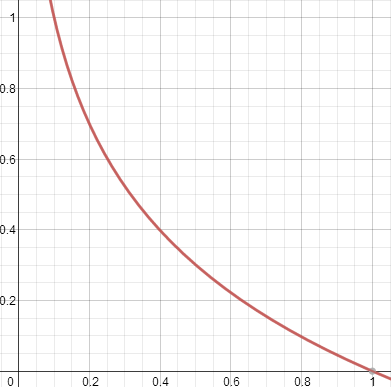
\includegraphics[width=2.5in]{yis1.png}\\
\end{minipage}
\begin{minipage}{3in}
{\small if $y=0$, \\}
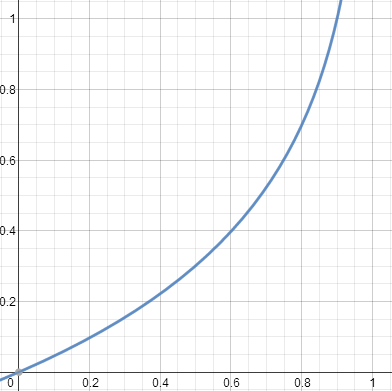
\includegraphics[width=2.5in]{yis0.png}\\
\end{minipage}

Notice that this cost function does a good job at giving the error between the predicted value and the true value. For example, if we predict that $h_{\theta} (x^{(i)}) = 1$ and $y = 1$, then by the graph on the left we see that the error is 0. On the other hand, if we predict that $h_{\theta} (x^{(i)}) = 0$ but $y = 1$, then the error diverges to infinity. Thus this function penalizes the learning algorithm with a very large cost on wrong predictions. The same argument applies to the graph on the right for $y=0$.\\

There is a clever way to re-write Cost$(h_{\theta} (x^{(i)}), y^{(i)})$ not as a piecewise function. Since either $y=0$ or $y=1$, then:
\[
\textnormal{Cost}(h_{\theta} (x^{(i)}), y^{(i)}) = 
-y^{(i)}\log(h_{\theta} (x^{(i)})) -(1 - y^{(i)})\log(1 - h_{\theta} (x^{(i)})) 
\textnormal{ .}
\]

This we have that the \emph{\color{red} logistic regression cost function} can be simply written as follows:

\[
\boxed{
C(\theta) = -\frac{1}{m}\sum\limits_{i=1}^m \left[y^{(i)}\log(h_{\theta} (x^{(i)})) +(1 - y^{(i)})\log(1 - h_{\theta} (x^{(i)}))\right]} \textnormal{ .}
\]

Now, with the correct cost function we can apply the gradient descent algorithm exactly as before:

\begin{framed}
{\bf Gradient Descent Algorithm} - We want to find the vector of parameters $\theta$ such that the cost function is minimized:\\

\noindent repeat until $C$ converges to a minimum \{\\
\indent for $j = 0,1,...,n$, simultaneously update:
\[
\theta_j := \theta_j - \alpha \frac{\partial}{\partial \theta_j} C(\theta)
\]
\}\\

where

\[
\frac{\partial}{\partial \theta_j}C(\theta) = \frac{1}{m}\sum\limits_{i=1}^m(h_{\theta}(x^{(i)})-y^{(i)})\cdot x^{(i)}
\]

and

\[
h_{\theta}(x^{(i)}) = \frac{1}{1+e^{-x^{(i)}\theta}}
\]

\end{framed}
\newpage

Notice that the derivative of the new cost function turns out to be exactly the same as the derivative of our old cost function (to see how this derivative was derived, please consult Professor's Ng \href{http://cs229.stanford.edu/notes/cs229-notes1.pdf}{lecture notes}). Also, as before you may need to scale and normalize the features in order for gradient descent to perform efficiently.

{\center\color{magenta}
\subsection*{\it\huge Brief Note: One-vs-All}}
\addcontentsline{toc}{subsection}{One-vs-All}
We have just learned about how to solve for 0-1 classification problems, but there are many classification problems out there that are not of the 0-1 type. For example, we may wish to implement email tagging that goes beyond spam versus ham and include other categories such as work, family, friends, etc.\\

As we have seen the way logistic regression works, we may feel restricted to only using it in cases where we wish to predict outcomes for two classes only. However, that is not the case. Along with a technique called ``one-vs-all'', we can use logistic regression to predict outcome for more than two classes.\\

One-vs-all is simply the technique of running multiple logistic regressions where in each run of logistic regression we pick only one of our classes to be the ``positive'' class (a different one each time), while the rest become the ``negative'' class. The logistic regression that outputs the \emph{highest} value of $h_{\theta}(x^{(i)})$ for some input $x^{(i)}$ ``wins'', that is we classify $x^{(i)}$ into the class $k$ where $k$ is the positive class in the respective logistic regression run.\\


{\center\color{magenta}
\subsection*{\it\huge An Example: Data Classification}}
\addcontentsline{toc}{subsection}{An Example: Data Classification}

We now turn our attention to the companion IJulia notebook for Lecture 8. There we shall explore the application of logistic regression to classify a group of candidates for admission at an university into two classes: accepted versus rejected. Using historical data from previous admission rounds, we will build a model to predict whether a an individual gets admitted based on their grades on two exams. Before we try to build our model, it may be useful to visualize our data:

\begin{center}
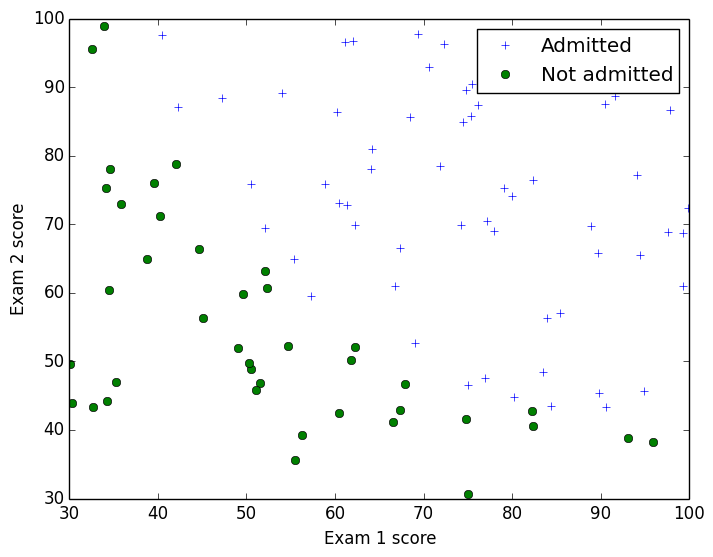
\includegraphics[width=5in]{admissions.png}\\
\end{center}


\newpage
\section*{Lecture 9}
\addcontentsline{toc}{section}{Lecture 9}

{\center\color{magenta}
\subsection*{\it\huge Recommender Systems}}
\addcontentsline{toc}{subsection}{Recommender Systems}

{\it\huge I}n this lecture we are going to explore a further application of linear regression: Recommender Systems. These are systems that allows businesses (or otherwise content providers) to more intelligently provide their content based on their customers preferences. For example, your ``movies-watched'' history on Netflix is input data for a recommender system that tries to predict what else you would like to watch, as it is in Netflix interest to keep you satisfied and watching. Another example is amazon.com, as they have a vast number of products and so it is in their interest to intelligently recommend you things that you are actually likely to buy.\\

There are two main types of recommender systems:
\begin{enumerate}
\item \emph{Content based systems: }these are systems that base recommendations on the content of the media or information. For example, if you watch actions movies on Netflix and rate those positively, chances are that you will enjoy other action movies.
\item \emph{Collaborative filtering systems: }these are systems that base recommendations on similarities amongst users or customers. For example, if you bought a book on amazon that another user also bought along with other books, then maybe you would like those other books too.\\
\end{enumerate}

Most recommender systems in use are based on these two main types or on some sort of hybrid of these types. There are many techniques from scientific computing and machine learning that can be applied to implement these different types of recommender systems - such as \href{https://en.wikipedia.org/wiki/Singular_value_decomposition}{singular value decomposition} and \href{https://en.wikipedia.org/wiki/Cluster_analysis}{clustering analysis} (which are not covered in this course). \\

Here, we will discuss simplified implementations of both content based and collaborative filtering systems that are basically applications of linear regression. We will focus on algorithms that use gradient-based optimization (such as gradient descent or some more advanced optimization algorithm like \href{https://en.wikipedia.org/wiki/L-BFGS}{L-BFGS}) to find the least squares solution. However, before we ``jump in'', let us take a detour through the topic of \emph{regularization}.\\

\begin{center}
\line(1,0){250}
\end{center}

{\color{red}\it\Large Regularization}\\

\emph{Regularization} refers to the technique of adding extra information to our linear (or logistic) regression in other to give preferential treatment to features that seem more relevantly correlated and penalize features whose correlation may not be that relevant to solving the regression (it can also be use to prevent over-fitting in polynomial regression - which we have not studies, but it is simply trying to find the polynomial of best fit, i.e. the degree of your polynomial solution can be greater than 1). \\

There are many \href{https://en.wikipedia.org/wiki/Regularization_(mathematics)}{ways} to perform regularization depending on the regression problem one is trying to solve. The regularization that we will use for our linear regression is this lecture is know as \href{https://en.wikipedia.org/wiki/Ridge_regression}{Tikhonov regularization}. I will leave the more conceptual and theoretical details to the reader to explore and simply state how our cost function and its derivative will be changed in the case of regularization.\\
\newpage

\begin{framed}
{\it Regularized Cost Function and its derivative:}
\[
C(\theta) = \frac{1}{2m}\left[\sum_{i = 1}^m(h_{\theta}(x^{(i)}) - y^{(i)})^2 + \lambda\sum_{j=1}^n \theta_j^2\right]
\]

for $j=0$:
\[
\frac{\partial}{\partial \theta_0}C(\theta) = \frac{1}{m}\sum_{i=1}^m(h_{\theta}(x^{(i)})-y^{(i)})x^{(i)}_0
\]

for $j > 0$:
\[
\frac{\partial}{\partial \theta_j}C(\theta) = \frac{1}{m}\sum_{i=1}^m(h_{\theta}(x^{(i)})-y^{(i)})x^{(i)}_j + \frac{\lambda}{m}\theta_j
\]
\end{framed}

$\lambda$ is called the \emph{regularization parameter} - it is a parameter we should tweak in order to reward (or penalize) certain features. Note that we do not regularize $\theta_0$ since it pertains to the ``ones'' feature and it is not affected by the weight of the features in consideration.

\begin{center}
\line(1,0){250}
\end{center}

{\center\color{magenta}
\subsection*{\it\huge Content Based Systems}}
\addcontentsline{toc}{subsection}{Content Based Systems}

{\it\huge I}n content based systems, the features which describe the content of something being recommended to users are known. However, the user weights for these features are not known. These features are information like amount of action or romance in a movie, or the different categories in which a particular product may fall. For example, if you search for ``scientific computing'' on amazon.com, you will get a list of books that fall in that category, but not only that, you will get a list in order of relevance. \\

Clicking one of the results and scrolling down a bit, we find yet another example of content based recommendations:

\begin{center}
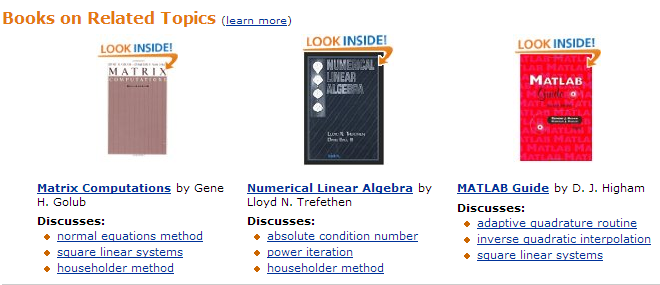
\includegraphics[scale=1]{cb.png}
\end{center}
\newpage

In order to introduce the topic and formulate the problem, let us work on a simplified example:

\begin{center}
\begin{tabular}{| c | c | c | c | c |}
\hline
Book & Alice & Bob & Charlie & Dave \\
\hline
Advanced Math in Greek & 5 & 0 & 5 & 0\\
\hline
The Book of Proofs & ? & 2 & 5 & 0\\
\hline
Down-to-Earth Math & 0 & 5 & 1 & 4\\
\hline
Everyday Math & 0 & ? & ? & ? \\
\hline
Intermediate Crazy Math & 5 & 0 & ? & ?\\
\hline
\end{tabular}
\end{center}

Say we have a matrix as above, where rows correspond to book tiles and columns correspond to readers (i.e. users of this system). An entry $a_{i,j}$ in this matrix is a number ranging from 0 through 5, representing the rating user $j$ gave to book $i$. If we do not have a rating from a particular user on a particular book, then the entry is represented by a ``?''. \\

\underline{Definitions:}
\begin{itemize}
\item $n_b$ is the number of books;
\item $n_u$ is the number of users;
\item $r(i,j) = 1$ if user $j$ has rated book $i$ (otherwise 0);
\item $y^{(i,j)}$ is the rating by user $j$ of book $i$ if $r(i,j) = 1$;
\item $\theta^{(j)}$ is the parameter vector for user $j$;
\item $x^{(i)}$ is the feature vector for book $i$; and 
\item $(\theta^{(j)})^T(x^{(i)})$ is thus, the predicted rating for user $j$, for book $i$.\\
\end{itemize}

Furthermore, in this case we know the feature vectors being considered: $x_1$ = amount of abstract mathematics and $x_2$ = amount of practical mathematics. That is, someone read all of these books and ``graded'' them on these features, say on a scale from 0.0 to 1.0. \\

In order for us to learn $\theta^{(j)}$ (the parameter vector for user $j$ - or the weights user $j$ gives to the features considered) we must solve the following optimization problem:

\[
\boxed{\min_{\theta^{(j)}} \left(\frac{1}{2} \sum_{i:r(i,j)=1}((\theta^{(j)})^T(x^{(i)}) - y^{(i,j)})^2 + \frac{\lambda}{2}\sum_{k=1}^n(\theta^{(j)}_k)^2\right)}
\]\\

Note that the expression inside the parenthesis looks just like the regularized cost function we mentioned earlier, with the exception of the division by $m$. Recall from our first discussion of linear regression that the $\frac{1}{m}$ constant multiplying our cost function was there for mathematical convenience and that it did not affect the minimum. Here, the analogous constant factor would be $\frac{1}{m^{(j)}}$ where $m^{(j)}$ is the number of books rated by user $j$. Since we will have to optimize for these $\theta^{(j)}$'s across all users $j$, then the constant factor $\frac{1}{m^{(j)}}$ is no longer convenient.\\

Thus to learn the parameters for all users $j$, that is $\theta^{(1)}, \theta^{(2)}, ..., \theta^{(n_u)}$, we need to solve:

\[
\boxed{\min_{\theta^{(1)}, \theta^{(2)}, ..., \theta^{(n_u)}} \left(\frac{1}{2} \sum_{j=1}^{n_u}\;\sum_{i:r(i,j)=1}((\theta^{(j)})^T(x^{(i)}) - y^{(i,j)})^2 + \frac{\lambda}{2}\sum_{j=1}^{n_u}\sum_{k=1}^n(\theta^{(j)}_k)^2\right)}\]\\

If we are using a gradient based optimization algorithm to solve for the above problem, then we provide the derivative of the cost function:

\begin{framed}
\noindent
For $k=0$ (since $j$ has a different meaning in our current formulation):
\[
\frac{\partial}{\partial \theta^{(j)}_0}C(\theta^{(j)}) = \sum_{i:r(i,j)=1}((\theta^{(j)})^T(x^{(i)}) - y^{(i,j)})x^{(i)}_0
\]

\noindent
and for $k > 0$:
\[
\frac{\partial}{\partial \theta^{(j)}_k}C(\theta^{(j)}) = \sum_{i:r(i,j)=1}((\theta^{(j)})^T(x^{(i)}) - y^{(i,j)})x^{(i)}_k + \lambda\theta^{(j)}_k
\]
\end{framed}

{\center\color{magenta}
\subsection*{\it\huge Collaborative Filtering Systems}}
\addcontentsline{toc}{subsection}{Collaborative Filtering Systems}

{\it\huge I}n collaborative filtering systems, the features which describe the content of something being recommended to users are not known. However, we do know the weights users give to particular features. For example, we know how Sally weighs her genre preferences when it comes to movies - we know that she really likes action movies, then ``contains action'' is a likely feature of the movies she watches.\\

On the same amazon.com page I was before, we find an example of collaborative filtering:\\

\begin{center}
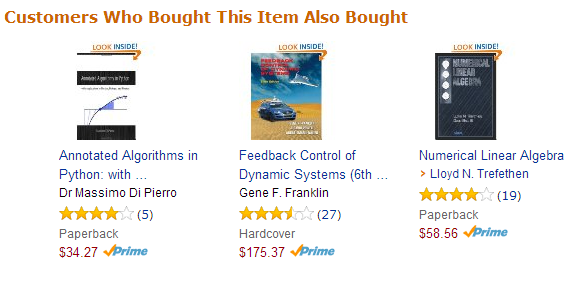
\includegraphics[scale=1]{cf.png}
\end{center}

Once again, let us work on a simplified example:

\begin{center}
\begin{tabular}{| c | c | c | c | c |}
\hline
Book & Alice & Bob & Charlie & Dave \\
\hline
Advanced Math in Greek & 5 & 0 & 5 & 0\\
\hline
The Book of Proofs & ? & 2 & 5 & 0\\
\hline
Down-to-Earth Math & 0 & 5 & 1 & 4\\
\hline
Everyday Math & 0 & ? & ? & ? \\
\hline
Intermediate Crazy Math & 5 & 0 & ? & ?\\
\hline
\end{tabular}
\end{center}

This is the same matrix as before, however now we do not have any tags on these books, i.e. there is no ``grade'' for the amount of abstract mathematics versus practical mathematics. However, we do have the following weight vectors for each user, say:\\

$\theta^{(1)} = \begin{bmatrix}
0\\ 5\\ 0
\end{bmatrix}, \; \theta^{(2)} = \begin{bmatrix}
0\\ 1\\ 5
\end{bmatrix}, \; \theta^{(3)} = \begin{bmatrix}
0\\ 5\\ 0
\end{bmatrix}, \; \theta^{(4)} = \begin{bmatrix}
0\\ 0\\ 5
\end{bmatrix}$\\

The definitions for the notation we will use here are the same as before. So given vectors $\theta^{(j)}$'s for all $n_u$ users, we wish to learn the vector $x^{(i)}$ (the feature vector for book $i$). Thus, we must solve the following optimization problem:

\[
\boxed{\min_{x^{(i)}} \left(\frac{1}{2} \sum_{j:r(i,j)=1}((\theta^{(j)})^T(x^{(i)}) - y^{(i,j)})^2 + \frac{\lambda}{2}\sum_{k=1}^n(x^{(i)}_k)^2\right)}
\]\\

In order to learn the features for all books $i$, that is $x^{(1)}, x^{(2)}, ..., x^{(n_b)}$, we need to solve:

\[
\boxed{\min_{x^{(1)}, x^{(2)}, ..., x^{(n_b)}} \left(\frac{1}{2} \sum_{i=1}^{n_b}\;\sum_{j:r(i,j)=1}((\theta^{(j)})^T(x^{(i)}) - y^{(i,j)})^2 + \frac{\lambda}{2}\sum_{i=1}^{n_b}\sum_{k=1}^n(x^{(i)}_k)^2\right)}\]\\

If we are using a gradient based optimization algorithm to solve for the above problem, then the derivative of the cost function here should be with respect to $x^{(i)}$, however it should not look too different from before and working the differentiation is left as an exercise to the reader.\\

So once we solve the above problem and get a good approximation of $x^{(1)}, x^{(2)}, ..., x^{(n_b)}$, there is no reason why we can't use this new information to estimate $\theta^{(1)}, \theta^{(2)}, ..., \theta^{(n_u)}$ - as we might not have all of them, or there may be new users over time. But there may also be new books over time, and we can go back and forth in this manner estimating features and parameters. \\

If you study the two minimization problems below, you will see that it is possible to combine them into one:\\

\begin{framed}
\noindent
In order to learn the features for all books $i$, that is $x^{(1)}, x^{(2)}, ..., x^{(n_b)}$, we need to solve:

\[
\min_{x^{(1)}, x^{(2)}, ..., x^{(n_b)}} \left(\frac{1}{2} \sum_{i=1}^{n_b}\;\sum_{j:r(i,j)=1}((\theta^{(j)})^T(x^{(i)}) - y^{(i,j)})^2 + \frac{\lambda}{2}\sum_{i=1}^{n_b}\sum_{k=1}^n(x^{(i)}_k)^2\right)\]\\

\noindent
In order to learn the parameters for all users $j$, that is $\theta^{(1)}, \theta^{(2)}, ..., \theta^{(n_u)}$, we need to solve:

\[
\min_{\theta^{(1)}, \theta^{(2)}, ..., \theta^{(n_u)}} \left(\frac{1}{2} \sum_{j=1}^{n_u}\;\sum_{i:r(i,j)=1}((\theta^{(j)})^T(x^{(i)}) - y^{(i,j)})^2 + \frac{\lambda}{2}\sum_{j=1}^{n_u}\sum_{k=1}^n(\theta^{(j)}_k)^2\right)\]\\

\noindent
... combined, becomes:
\[
\min_{x^{(1)}, x^{(2)}, ..., x^{(n_b)}, \theta^{(1)}, \theta^{(2)}, ..., \theta^{(n_u)}} \left(\frac{1}{2} \sum_{(i,j):r(i,j)=1}((\theta^{(j)})^T(x^{(i)}) - y^{(i,j)})^2 + \frac{\lambda}{2}\sum_{i=1}^{n_b}\sum_{k=1}^n(x^{(i)}_k)^2 + \frac{\lambda}{2}\sum_{j=1}^{n_u}\sum_{k=1}^n(\theta^{(j)}_k)^2\right)\]

\end{framed}

\newpage

So to implement collaborative filtering:
\begin{enumerate}
\item Initialize $x^{(1)}, x^{(2)}, ..., x^{(n_b)}, \theta^{(1)}, \theta^{(2)}, ..., \theta^{(n_u)}$ to small random numbers.
\item Minimize the cost function 
\[C(x^{(1)}, x^{(2)}, ..., x^{(n_b)}, \theta^{(1)}, \theta^{(2)}, ..., \theta^{(n_u)}) = \frac{1}{2} \sum_{(i,j):r(i,j)=1}((\theta^{(j)})^T(x^{(i)}) - y^{(i,j)})^2 + \frac{\lambda}{2}\sum_{i=1}^{n_b}\sum_{k=1}^n(x^{(i)}_k)^2 + \frac{\lambda}{2}\sum_{j=1}^{n_u}\sum_{k=1}^n(\theta^{(j)}_k)^2\] 
using gradient descent or another optimization algorithm.
\item For a user $j$ with parameters $\theta^{(j)}$ and for a book $i$ with features $x^{(i)}$, predict a rating of $(\theta^{(j)})^T(x^{(i)})$.
\end{enumerate} 

The algorithm just described here is also known as \emph{low-rank matrix factorization}, due to the vectorized implementation of the predicted ratings $X\Theta^T$ being a matrix of low-rank.\\

We can use the results to find the top five similar books to some book $i$ as follows: find the five books $l$ with the smallest distance from book $i$, that is $||x^{(i)} - x^{(l)}||$.

\newpage
\section*{Lecture 10}
\addcontentsline{toc}{section}{Lecture 10}
\subsection*{\it\huge Activity and Conclusion}
\addcontentsline{toc}{subsection}{Activity and Conclusion}
{\bf Note: }The activity will be available in class only, during the last class.

\end{document}